\documentclass[10pt,a4paper]{article}
\usepackage[T1]{fontenc}
\usepackage[utf8]{inputenc}
\usepackage{lmodern}
\usepackage{microtype}
\usepackage[margin=2.2cm,headheight=14pt]{geometry}
\usepackage{amsmath,amssymb,bm}
\usepackage{graphicx}
\usepackage{booktabs,tabularx,array}
\usepackage[table]{xcolor}
\usepackage{tikz}
\usetikzlibrary{arrows.meta,positioning}
\usepackage{float}
\usepackage[font=small,labelfont=bf]{caption}
\usepackage{algorithm}
\usepackage{algpseudocode}
\usepackage{enumitem}
\usepackage{titlesec}
\usepackage{fancyhdr}
\usepackage[most]{tcolorbox}
\usepackage[colorlinks=true,linkcolor=bpdeep,urlcolor=bp]{hyperref}
\definecolor{bp}{HTML}{1E5AA8}
\definecolor{bpdeep}{HTML}{123A6E}
\definecolor{bpwash}{HTML}{EAF1FA}
\definecolor{amber}{HTML}{9C6B0B}
\definecolor{okc}{HTML}{1E7B3A}
\definecolor{failc}{HTML}{B22222}
\definecolor{muted}{HTML}{5B6670}
\titleformat{\section}{\Large\bfseries\color{bpdeep}}{\thesection}{0.8em}{}
\titleformat{\subsection}{\large\bfseries\color{bpdeep}}{\thesubsection}{0.7em}{}
\setlength{\parskip}{0.4em}
\setlength{\parindent}{0pt}
\setlist{nosep,leftmargin=1.5em}
\renewcommand{\arraystretch}{1.15}
\pagestyle{fancy}
\fancyhf{}
\lhead{\small\color{muted}Layout optimization algorithms}
\rhead{\small\color{muted}\thepage}
\renewcommand{\headrulewidth}{0.3pt}
\newcommand{\code}[1]{\texttt{\small #1}}
\newtcolorbox{example}[1]{enhanced,breakable,colback=bpwash,colframe=bp,boxrule=0.5pt,arc=2pt,
  left=6pt,right=6pt,top=4pt,bottom=4pt,fonttitle=\bfseries\small,title={Worked example: #1}}
\newtcolorbox{note}{enhanced,breakable,colback=amber!8,colframe=amber,boxrule=0.5pt,arc=2pt,left=6pt,right=6pt,top=4pt,bottom=4pt}
\tikzset{box/.style={draw=bpdeep, fill=bpwash, rounded corners=2pt, align=center, font=\footnotesize, minimum height=9mm,
  inner sep=3pt}, arr/.style={-{Stealth[length=2mm]}, thick, bpdeep}}
\begin{document}


\begin{titlepage}\centering
\vspace*{1.5cm}
{\color{bpdeep}\rule{\linewidth}{1.2pt}}\par\vspace{0.6cm}
{\huge\bfseries\color{bpdeep} How the Layout Optimization\\[0.3em] Algorithms Work}\par\vspace{0.5cm}
{\large The reference genetic algorithm, the updated genetic algorithm, the systematic search\\
and the hotel layout exploration, each with worked examples}\par\vspace{0.4cm}
{\color{bpdeep}\rule{\linewidth}{1.2pt}}\par\vspace{1.0cm}
{\large Naimul Haque}\par{\normalsize Semester project with RNGD}\par\vspace{0.3cm}{\normalsize October 2026}\par
\vspace{1.0cm}
\begin{minipage}{0.88\linewidth}\small
\textbf{What this report is.} A step-by-step explanation of the optimization algorithms in the RNGD AI Studio. It
covers only the algorithms: what they search over, how one candidate layout is built and scored, and how each search
moves from one candidate to the next. Every step is followed by an example with real numbers.

\textbf{Where the examples come from.} All examples were computed by the code itself on one case and written into this
report by a script, so they can be reproduced:
\begin{itemize}
\item site \code{fp1} of RNGD's design-optimization prototype (3 levels, 9,640 SF placeable per level,
2 cores) with the prototype's hotel program (72 rooms, 69 of them guest rooms);
\item search budget 24 $\times$ 30 $=$ 720 layouts, random seed 7, no language model anywhere;
\item for the hotel sections, the Project Renegade Living\,+\,Lodging program (117 keys).
\end{itemize}

\textbf{The short version.}
\begin{enumerate}
\item No algorithm here moves rooms around directly. Each one searches over a short list of numbers (a \emph{genome}),
and a fixed procedure (the \emph{decoder}) turns that list into a complete floor plan, which is then scored (the
\emph{fitness}).
\item The reference genetic algorithm (GA) and my first attempt let corridor segments sit anywhere. Their plans left
guest rooms without windows.
\item The updated decoder only builds plans an architect would accept: straight corridors one room depth from the
facade, rooms in modular bays, a window for every guest room. On the example site it places 72 of 72
rooms where the reference placed 61.
\item Two searches drive that decoder: a genetic algorithm with local search, and a deterministic search that
enumerates corridor combinations and then improves the best ones move by move. The second is the default.
\item In the hotel mode an outer loop also generates the building shape, the core position and the floor count, and a
separate ranking step (Pareto front and TOPSIS) orders the layouts found.
\end{enumerate}
\end{minipage}
\vfill
{\small\color{muted} Built 2026-10-11 22:02 from \code{reports/optimization/examples.json}.}
\end{titlepage}
\tableofcontents
\clearpage


\section{The problem and the running example}
\subsection{What has to be decided}
A site is a stack of levels. Each level is a grid of 1\,ft cells, and every cell is one of: \emph{placeable},
\emph{core} (stairs and elevators), \emph{structure} or \emph{outside}. A program lists the rooms to place: a size,
a count, a priority and a few flags (needs a window, should be near a core, one per floor).

A layout answers two questions:
\begin{itemize}
\item \textbf{Where is the corridor?} A set of placeable cells, the same on every level so that the floors stack.
\item \textbf{Where is each room?} A rectangle on one level, opening onto the corridor, not overlapping anything.
\end{itemize}
The layout should place as many rooms as possible, give guest rooms a window, keep the corridor short, satisfy the
egress rules, and so on. Section~\ref{sec:fitness} turns that list into one number, the fitness $F$.

\subsection{The running example}
The example used throughout is site \code{fp1}: an L-shaped plate of 151 $\times$ 100 cells, 3
levels (L1, L2, L3), 9,640 SF placeable per level and 2 cores. The program is
\code{QA/rooms\_hotel.json}:
\begin{table}[H]\centering\small\caption{The example program. Category, window and near-core flags are inferred from the room name.}\label{tab:program}
\begin{tabular}{@{}l c r r r l c c@{}}
\toprule
\textbf{Room type} & \textbf{Size, ft} & \textbf{Area, SF} & \textbf{Instances} & \textbf{Priority} & \textbf{Category} & \textbf{Window} & \textbf{Near core} \\ \midrule
King & 25 $\times$ 12 & 300 & 63 & 2 & guest & yes & no \\
ADA corner suite & 30 $\times$ 24 & 720 & 3 & 5 & ada & yes & yes \\
ADA suite & 25 $\times$ 20 & 500 & 3 & 3 & ada & yes & yes \\
Janitor's closet & 25 $\times$ 10 & 250 & 3 & 10 & service & no & yes \\
\bottomrule
\end{tabular}
\end{table}
The janitor's closet is one per floor, so the program has 72 room instances in total, 69 of them keys.

\begin{figure}[H]\centering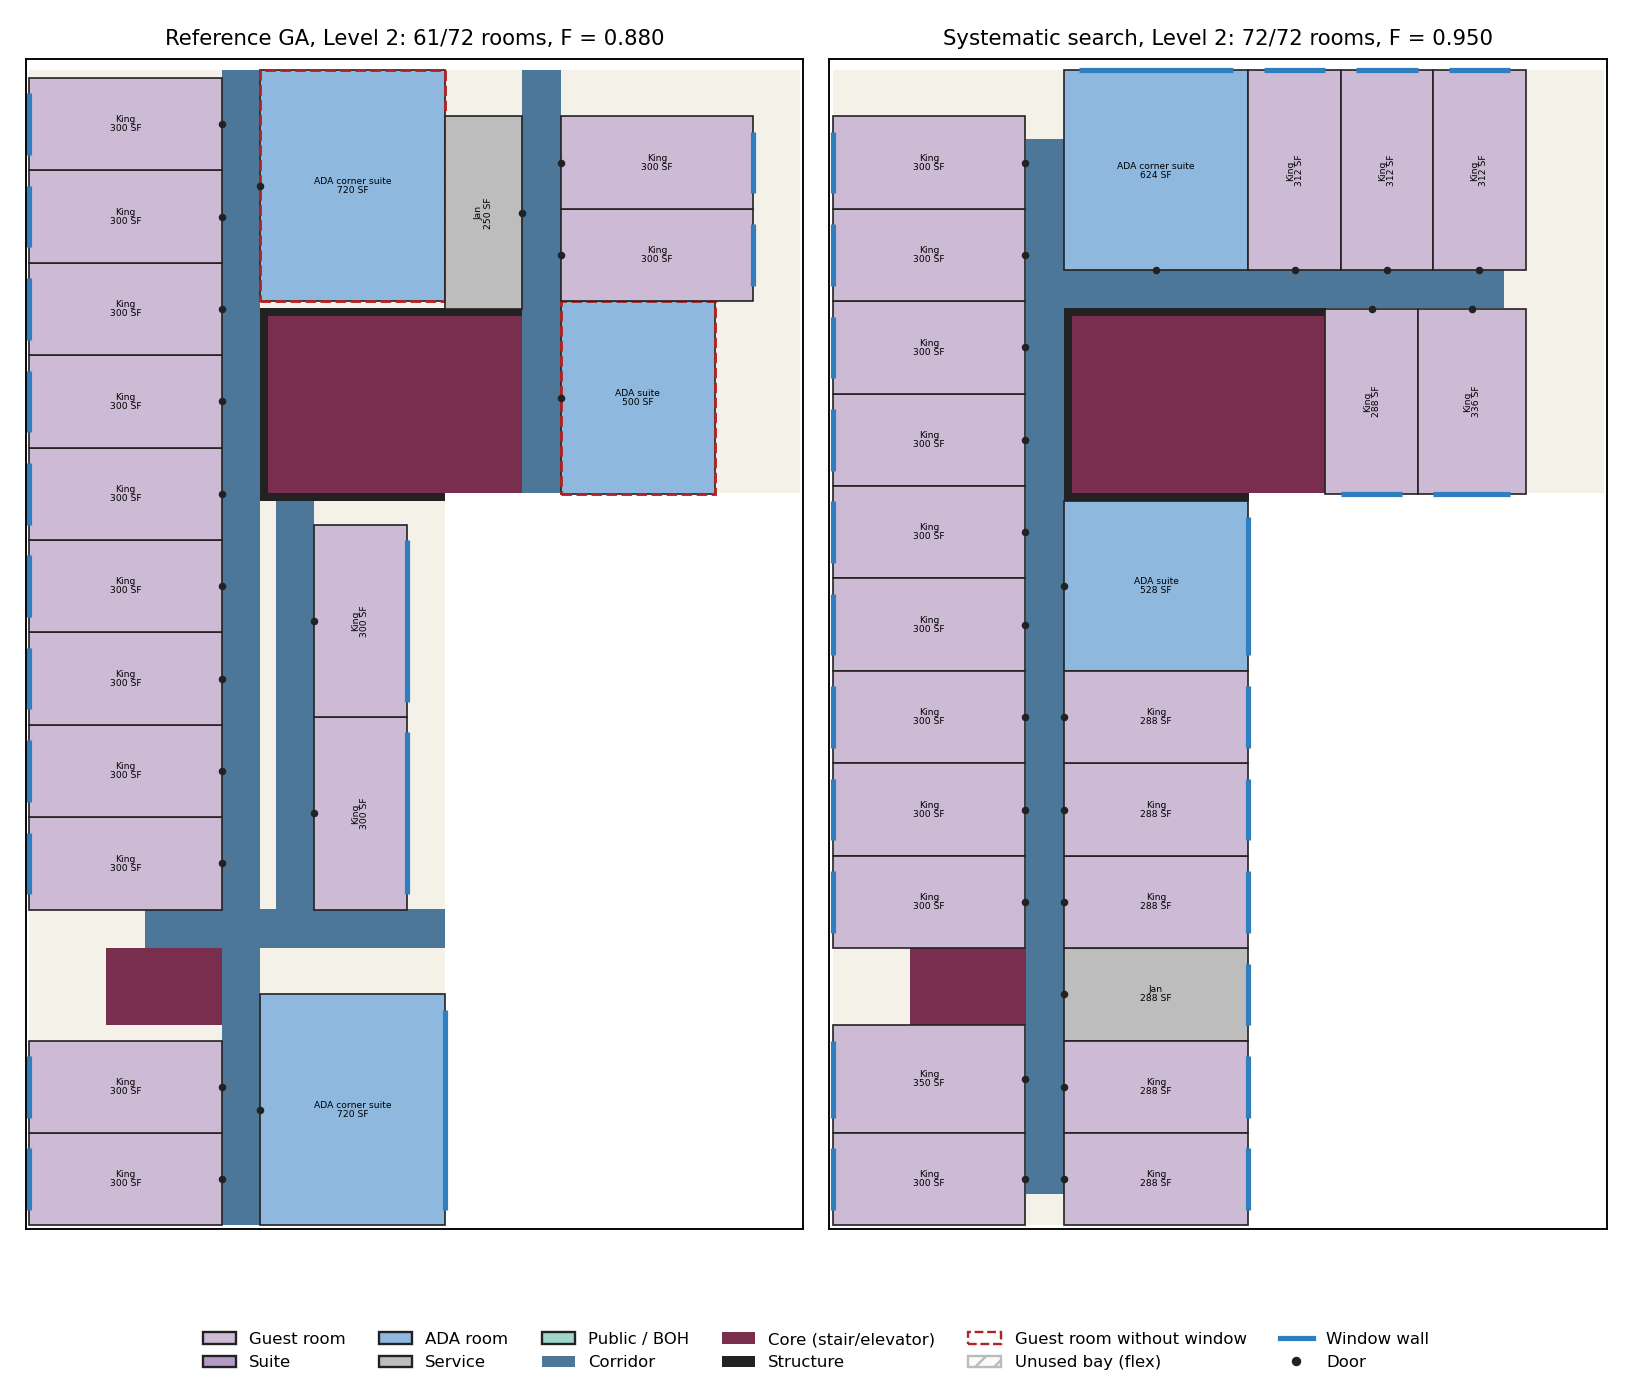
\includegraphics[width=\linewidth,height=0.42\textheight,keepaspectratio]{before_after.png}\caption{The running example, Level 2. Left: the layout delivered by the reference GA. Right: the layout found by the systematic search with the updated decoder. A red dashed outline marks a guest room without a window; blue lines are window walls.}\end{figure}

\subsection{Why the search does not move rooms directly}
The number of ways to put 72 rectangles on a 151 $\times$ 100 grid is astronomically large, and almost
all of them are useless: rooms overlap, have no door on a corridor, or sit in the middle of the plate. All the
algorithms in this report therefore share one structure (Figure~\ref{fig:loop}):
\begin{enumerate}
\item the search proposes a \textbf{genome}, a short vector of numbers between 0 and 1;
\item a \textbf{decoder} turns the genome into a complete layout by fixed rules;
\item the \textbf{fitness} scores that layout;
\item the search uses the score to propose the next genome.
\end{enumerate}
The algorithms differ in two places only: what the decoder does (Sections~\ref{sec:ref}, \ref{sec:free} and
\ref{sec:decoder}), and how the search proposes the next genome (Sections~\ref{sec:ga} and \ref{sec:sys}).

\begin{figure}[H]\centering
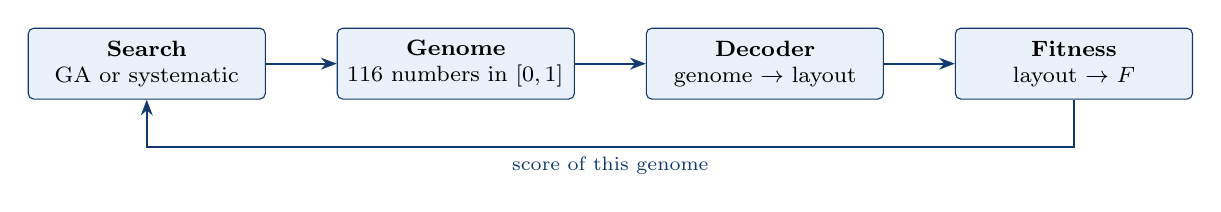
\begin{tikzpicture}[node distance=9mm]
\node[box, text width=28mm] (s) {\textbf{Search}\\GA or systematic};
\node[box, text width=28mm, right=of s] (g) {\textbf{Genome}\\116 numbers in $[0,1]$};
\node[box, text width=28mm, right=of g] (dcd) {\textbf{Decoder}\\genome $\to$ layout};
\node[box, text width=28mm, right=of dcd] (f) {\textbf{Fitness}\\layout $\to$ $F$};
\draw[arr] (s) -- (g); \draw[arr] (g) -- (dcd); \draw[arr] (dcd) -- (f);
\draw[arr] (f.south) -- ++(0,-6mm) -| node[pos=0.25, below, font=\scriptsize]{score of this genome} (s.south);
\end{tikzpicture}
\caption{The loop shared by all the algorithms. For the running example the genome has 116 numbers.}\label{fig:loop}
\end{figure}

\begin{table}[H]\centering\small\caption{The algorithms covered in this report.}\label{tab:algs}
\begin{tabular}{@{}l p{3.3cm} p{4.3cm} p{4.6cm} p{2.3cm}@{}}
\toprule
\textbf{} & \textbf{Algorithm} & \textbf{Decoder} & \textbf{Search} & \textbf{Same result every run} \\ \midrule
A & Reference GA (prototype) & free corridor genes & genetic algorithm, 500 generations & not recorded \\
B & First attempt & free corridor segments, greedy packer & memetic GA & yes (seeded) \\
C & Updated GA & architectural decoder & memetic GA & yes (seeded) \\
D & Systematic search (default) & architectural decoder & enumeration, pattern search, iterated local search & yes \\
E & Hotel exploration & architectural decoder on generated plates & enumeration of plates, pattern search & yes \\
\bottomrule
\end{tabular}
\end{table}


\section{Algorithm A: the reference genetic algorithm}\label{sec:ref}
\begin{note}
I have the reference GA's \emph{result files} (\code{QA/floorplan1--3.json}), not its source code. This section
describes what those files record and what can be measured from them. It does not guess at internals.
\end{note}

\subsection{What a genetic algorithm does}
A genetic algorithm keeps a \emph{population} of candidate genomes. In every \emph{generation} it
\begin{enumerate}
\item scores every candidate,
\item \emph{selects} better candidates as parents,
\item makes children by \emph{crossover} (taking some genes from one parent and some from the other),
\item \emph{mutates} the children (small random changes),
\item and replaces the population with the children, usually keeping the best old candidates (\emph{elitism}).
\end{enumerate}
Good gene combinations survive and spread; mutation keeps introducing new ones.

\subsection{What the result files record}
\begin{itemize}
\item \textbf{A corridor genome.} A list of corridor genes, each three integers. For \code{fp1} there are
12 genes; the first three are (190, 1, 43), (51, 1, 101), (1994, 3, 105). The corridor they produce is stored as a list of cells
(corridor width 5\,ft, the same on all levels).
\item \textbf{Room placements.} For each placed room: level, anchor cell, the side it faces, frontage and depth.
\item \textbf{A history.} One entry per generation with two numbers: the rooms not yet placed and a score. All three
runs have 500 entries.
\item \textbf{Settings.} A seed, an adjacency weight (0.15) and a balance weight (0.0).
\end{itemize}
\begin{table}[H]\centering\small\caption{The three reference runs, as recorded in their result files.}\label{tab:ref}
\begin{tabular}{@{}l r r r r r r r@{}}
\toprule
\textbf{Site} & \textbf{Genes} & \textbf{Generations} & \textbf{Unplaced, start} & \textbf{Unplaced, end} & \textbf{Last improvement} & \textbf{Placed} & \textbf{Seed} \\ \midrule
fp1 & 12 & 500 & 36 & 11 & 467 & 61/72 & 5 \\
fp2 & 9 & 500 & 42 & 19 & 407 & 53/72 & 6 \\
fp3 & 7 & 500 & 34 & 15 & 126 & 57/72 & 1 \\
\bottomrule
\end{tabular}
\end{table}
\begin{figure}[H]\centering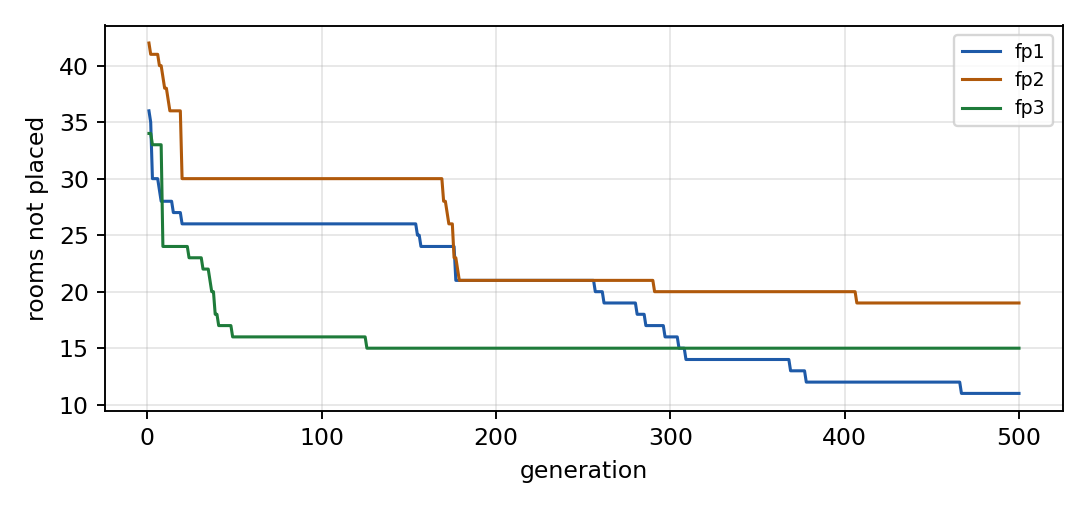
\includegraphics[width=0.7\linewidth,height=0.28\textheight,keepaspectratio]{reference_history.png}\caption{Reference GA: rooms not placed in each of the 500 generations (from the history stored in the result files).}\end{figure}

\begin{example}{reading the history of \code{fp1}}
The run starts with 36 of 72 rooms unplaced and ends with 11 unplaced, so 61 rooms are placed. The
last improvement happens in generation 467 of 500: for the remaining 33 generations the best plan does not
change.
\end{example}

\subsection{What goes wrong, measured}
I rebuilt each delivered layout cell by cell and scored it with the fitness of Section~\ref{sec:fitness}, the same one
used for every other algorithm. For \code{fp1}:
\begin{itemize}
\item 61 of 72 rooms are placed;
\item 7 guest rooms have no window, although the file reports an exterior fraction of 1.0
(the two measures differ: mine counts a window only if at least half of the room's back wall lies within 6\,ft of
the facade);
\item 15\% of the placeable area is corridor and 16\% is neither room nor corridor;
\item its fitness is $F = 0.880$.
\end{itemize}
The cause is the representation. A corridor gene can put a corridor segment anywhere on the plate, and rooms are then
attached wherever they touch a corridor. Nothing in the genome knows where the facade is, so whether a room gets a
window is left to chance, and the gaps between rooms are too irregular to use. Longer runs do not fix this:
the search is looking in a space where almost every candidate is a poor plan.


\section{Algorithm B: my first attempt (free-form corridors)}\label{sec:free}
My first optimizer kept the reference idea and improved the parts around it. It is described here because it shows
that better scoring and a better search were not enough.

\subsection{Genome and decoder}
The genome has 10 corridor segments of four genes each, then one \emph{order key} per room:
\begin{itemize}
\item \textbf{Segment genes} $(u, v, o, \ell)$. The segment starts at the placeable cell nearest to column $u \cdot
(\text{cols}-1)$ and row $v \cdot (\text{rows}-1)$. It is horizontal if $o < 0.5$, otherwise vertical. It grows both
ways by up to $\ell \cdot \text{span}/2$ cells while the corridor width stays placeable. A segment with $\ell < 0.12$
is switched off.
\item \textbf{Repair.} All corridor pieces and all cores are joined into one network by least-cost paths.
\item \textbf{Order keys.} Rooms are placed in decreasing order of $0.06 \cdot \text{priority} + \text{key}$.
\item \textbf{Greedy packing.} Each room in turn is put at the best free position that touches the corridor. Positions
are scored for a window, a corner, distance to a core and how tightly the room sits against its neighbours.
\end{itemize}

\begin{example}{decoding one segment}
One of the seed genomes has a single active segment $(u, v, o, \ell) = (0.5, 0.81, 0.0, 1.0)$ on the
151 $\times$ 100 grid:
\begin{itemize}
\item start near column $0.5 \times 99 \approx 50$ and row $0.81 \times 150 \approx 122$;
\item $o = 0.0 < 0.5$, so it runs horizontally;
\item reach $= 1.0 \times 100 / 2 = 50$ cells each way, cut short where the plate ends.
\end{itemize}
Packing the 72 rooms around this corridor places 50 of them, 3 guest rooms without a window, for a
fitness of 0.820 (Figure~\ref{fig:free}).
\end{example}
\begin{figure}[H]\centering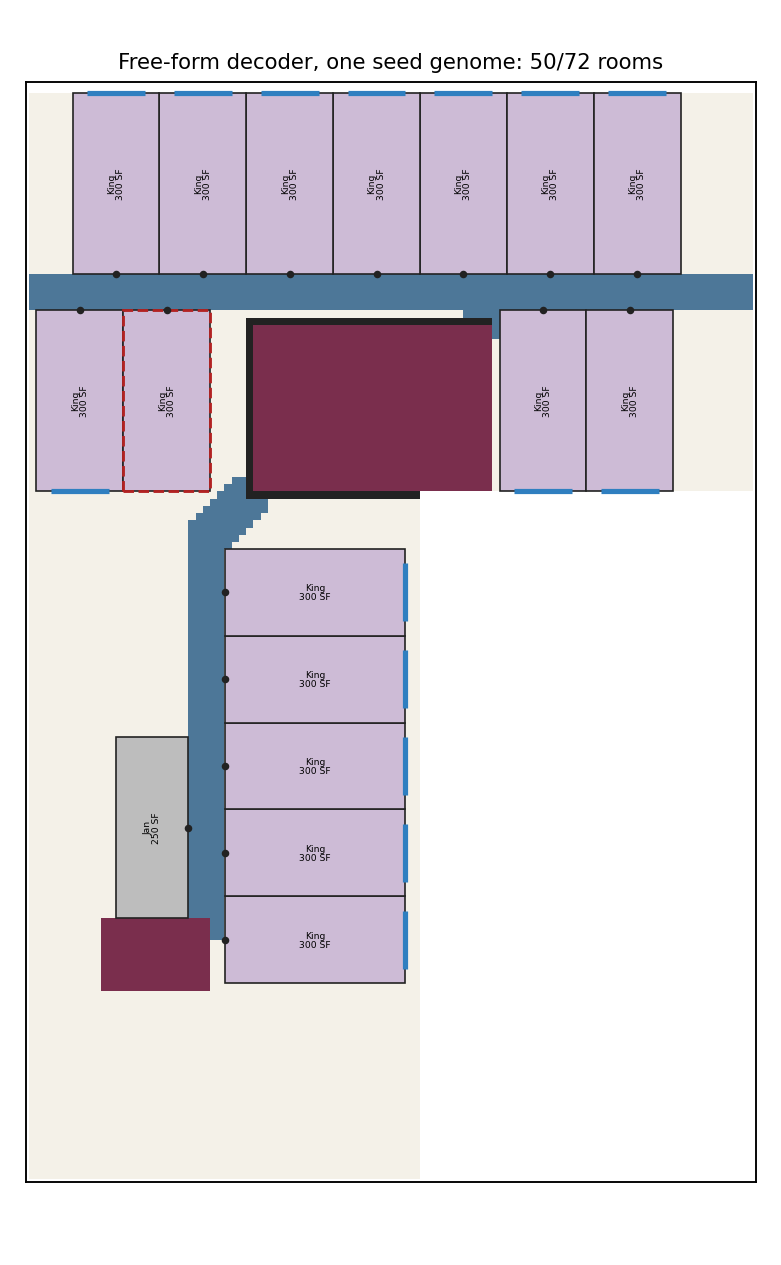
\includegraphics[width=0.42\linewidth,height=0.36\textheight,keepaspectratio]{freeform_seed.png}\caption{The free-form decoder on one seed genome (Level 2).\label{fig:free}}\end{figure}

\subsection{Result and lesson}
With a memetic GA around this decoder (the same search as Section~\ref{sec:ga}) and the full budget, the example site
reached 53 of 72 rooms with 3 windowless guest rooms and $F = 0.880$, in 119\,s. Over the three
sites it placed 174 rooms against the reference's 171, with 14 windowless guest rooms against
24. The scoring was better and the search was seeded and repeatable, but the plans still had the same faults.
The representation had to change.


\section{The architectural decoder (used by C, D and E)}\label{sec:decoder}
The updated decoder builds a floor plan the way a hotel floor is normally laid out. The search no longer decides
\emph{where corridor cells are}. It decides \emph{which of a few sensible corridors exist} and \emph{in which order
rooms claim their places}. This section follows one genome through all seven steps: the genome of the best layout the
systematic search found for the running example.

\subsection{Step 1: the bay module}
All rooms are placed on a grid of \emph{bays} along the corridor. One bay is one standard guest-room frontage wide.
\begin{itemize}
\item The module $M$ is the \textbf{weighted median} of the guest-room frontages, weighted by room count (a suite
counts as half its frontage, since it takes two bays).
\item $D$ is the median guest-room depth; $D_{\min} = \lfloor 0.92\, d_{\min} \rfloor$ is the shallowest strip a room may
use; $D_{\max} = d_{\max} + 2$ the deepest.
\end{itemize}
\begin{example}{module of the example program}
Guest-room frontages (the shorter side of each room): King 12\,ft ($\times$63); ADA corner suite 24\,ft ($\times$3); ADA suite 20\,ft ($\times$3). Sorted by frontage, the middle one of the 69 guest
rooms is a King, so $M = 12$\,ft. Depths are 25, 30, 25\,ft, so $D = 25$\,ft, $D_{\min} = \lfloor 0.92 \times 25 \rfloor =
23$\,ft and $D_{\max} = 32$\,ft. The corridor is $w = 5$\,ft wide. One bay is therefore
$12 \times 25 = 300$\,SF.
\end{example}

\subsection{Step 2: candidate spines}
A \emph{spine} is a straight corridor line: a row (horizontal corridor) or a column (vertical corridor). Every row and
column $k$ of the plate that can hold a corridor band gets a score
\[ s(k) = \sum_{x \in \text{band}(k)} \big[\, g_a(x) + g_b(x) + 1.5\,n_a(x) + 1.5\,n_b(x) + 0.5\,r_a(x) + 0.5\,r_b(x) \,\big]. \]
At each foot $x$ along the line, and for each of its two sides $a$ and $b$:
\begin{itemize}
\item $g = 1$ if a room at least $D_{\min}$ deep fits on that side;
\item $n = 1$ if, in addition, the facade is about one room depth away (at most $D + 2 +$ slack), so a room there has
a window;
\item $r = 1$ if the facade is within the deepest room's depth.
\end{itemize}
So one foot of corridor with window rooms on both sides scores $2 \times (1 + 1.5 + 0.5) = 6$, with window rooms on one
side only $3$, and with deep windowless space on both sides $2$.

In each direction the best lines are taken in order of score, skipping any line closer than $D_{\min} + w$ to one
already chosen (two corridors that close would leave no room between them). The ten best pieces overall become the
candidates. A plate may have fewer than ten.

\begin{example}{candidate spines of \code{fp1}}
The plate has $m = 5$ candidates (Figure~\ref{fig:scores}, Table~\ref{tab:cands}). Spine 0 is the column one room
depth in from the long west facade: it scores 733 over 150\,ft, or 4.89 per foot, close to the maximum of 6.
The lowest-ranked spine scores 2.00 per foot.
\end{example}
\begin{table}[H]\centering\small\caption{Candidate spines of \code{fp1}, best first.}\label{tab:cands}
\begin{tabular}{@{}c l r c r r r@{}}
\toprule
\textbf{Spine} & \textbf{Direction} & \textbf{Row / column} & \textbf{Extent} & \textbf{Length, ft} & \textbf{Score $s$} & \textbf{Score per ft} \\ \midrule
0 & vertical (column) & 27 & 0--149 & 150 & 733 & 4.89 \\
1 & horizontal (row) & 121 & 0--99 & 100 & 438 & 4.38 \\
2 & vertical (column) & 74 & 95--149 & 55 & 196 & 3.56 \\
3 & horizontal (row) & 27 & 25--53 & 29 & 116 & 4.00 \\
4 & horizontal (row) & 66 & 0--53 & 54 & 108 & 2.00 \\
\bottomrule
\end{tabular}
\end{table}
\begin{figure}[H]\centering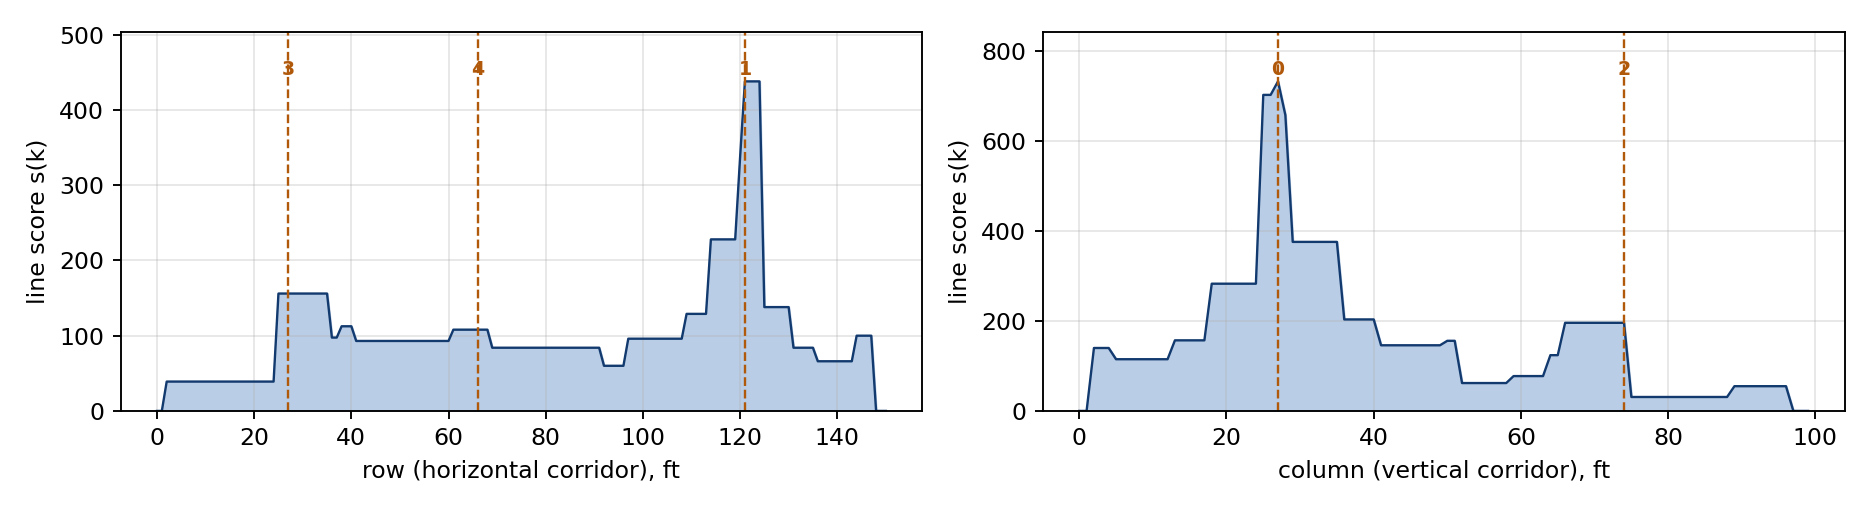
\includegraphics[width=\linewidth,height=0.24\textheight,keepaspectratio]{line_scores.png}\caption{The line score $s(k)$ of every row and every column of \code{fp1}. Dashed lines mark the candidates chosen (numbered as in Table~\ref{tab:cands}).\label{fig:scores}}\end{figure}

\subsection{Step 3: from genome to active spines}
For 72 rooms the genome has $10 \times 4 + 4 + 72 = 116$ numbers:
\begin{itemize}
\item \textbf{ten spine blocks} of four genes: trim at the low end, trim at the high end, shift, and an on/off gene
(the spine is on if that gene is at least 0.12);
\item \textbf{four connector genes}, which choose the elbow direction of L-shaped connectors;
\item \textbf{one order key per room}.
\end{itemize}
Blocks for candidates the plate does not have are simply ignored (here blocks 5 to 9).

A shift gene $h$ moves the line sideways by $\operatorname{round}(4(h - 0.5))$\,ft, so by at most 2\,ft. If the shifted
line would hit an obstacle, the scored position is kept. A trimmed spine shorter than $2M$ is dropped.

\begin{example}{the spine genes of the example genome}
\begin{center}\centering\small
\begin{tabular}{@{}c r r r r l@{}}
\toprule
\textbf{Spine} & \textbf{Trim low} & \textbf{Trim high} & \textbf{Shift} & \textbf{On/off gene} & \textbf{State} \\ \midrule
0 & 0.00 & 0.00 & 0.50 & 1.00 & on \\
1 & 0.00 & 0.30 & 0.50 & 1.00 & on \\
2 & 0.00 & 0.00 & 0.50 & 1.00 & on \\
3 & 0.00 & 0.00 & 0.50 & 1.00 & on \\
4 & 0.00 & 0.00 & 0.50 & 1.00 & on \\
\bottomrule
\end{tabular}
\end{center}
Spine 1 runs from 0 to 99 ($n = 100$\,ft) and has trim genes
$(0.00, 0.30)$. The low end moves in by $\lfloor 0.00 \times 0.35 \times 100 \rfloor = 0$\,ft and the
high end by $\lfloor 0.30 \times 0.35 \times 100 \rfloor = 10$\,ft, so it becomes 0--89. A trim
gene can remove at most 35\% of a spine from each end. All shift genes are 0.5, so no line moves.
\end{example}

\subsection{Step 4: trimming to the rooms and connecting}
\begin{enumerate}
\item A first pass builds bays along every active spine (Step 5) and \textbf{cuts each spine back to its own bays}, so
no corridor runs past the last possible room. A spine that ends up with no bays of its own is dropped.
\item The remaining spines and all cores are joined into one network. The nearest unconnected piece is linked by an
\textbf{L-shaped path}: one horizontal and one vertical leg, never a diagonal. A connector gene picks which leg comes
first. If both L-shapes are blocked, a rectilinear least-cost path is used.
\item Pieces that still cannot be reached are removed.
\end{enumerate}
\begin{example}{corridor of the example genome}
All 5 spines are switched on, but after the first pass the corridor consists of: column 27, 0--149 (150\,ft); row 121, 30--89 (60\,ft). The other spines
received no bays of their own and were dropped. These spines occupy 1,050 corridor cells and the connectors add
0: here the two spines cross and both cores lie on them, so no connector is needed. The corridor reaches
2 of 2 cores.
\end{example}

\subsection{Step 5: bays}
Each side of each straight corridor run is cut into bays of width $M$:
\begin{itemize}
\item a run of length $\ell$ gives $n = \lfloor \ell / M \rfloor$ full bays;
\item a remainder $\rho = \ell - nM$ smaller than $0.4M$ is absorbed by the last bay (a wider end bay, which suits a
suite); a larger remainder becomes a narrow bay of its own (for a service room);
\item a bay's depth is the free depth behind it, capped at $D_{\max}$;
\item a bay \textbf{has a window} if its back wall is on the facade, and is a \textbf{corner} bay if a side wall is too.
\end{itemize}
Bays are built in \textbf{two passes over all corridors}: first every bay that has a window, then windowless bays in
whatever space is left. Without this, the windowless inner side of one corridor could take the strip of floor that
another corridor needs for its window rooms.

Every level gets the same bays, which is what makes the floors stack.

\begin{example}{bays of the example layout}
There are 27 bays per floor: 27 with a window, 0 without, 3 on a corner. Some of the runs:
\begin{itemize}
\item A run of 114\,ft facing W: $\lfloor 114/12 \rfloor = 9$ full bays, remainder $6 \ge 4.8$\,ft, so it becomes a narrow bay of its own. Bay widths: 12, 12, 12, 12, 12, 12, 12, 12, 12, 6\,ft; depth 25\,ft.
\item A run of 94\,ft facing E: $\lfloor 94/12 \rfloor = 7$ full bays, remainder $10 \ge 4.8$\,ft, so it becomes a narrow bay of its own. Bay widths: 12, 12, 12, 12, 12, 12, 12, 10\,ft; depth 24\,ft.
\item A run of 60\,ft facing N: $\lfloor 60/12 \rfloor = 5$ full bays, no remainder. Bay widths: 12, 12, 12, 12, 12\,ft; depth 26\,ft.
\item A run of 26\,ft facing W: $\lfloor 26/12 \rfloor = 2$ full bays, remainder $2 < 0.4 \times 12 = 4.8$\,ft, so the last bay absorbs it and is 14\,ft wide. Bay widths: 12, 14\,ft; depth 25\,ft.
\end{itemize}
\end{example}

\subsection{Step 6: assigning rooms to bays}
\textbf{Order.} Rooms are taken in decreasing order of
\[ 0.06 \times \text{priority} + \text{order key}. \]
With all keys equal (0.5), this is pure priority order. The search changes the order by changing keys.

\textbf{Bays per room.} A room of nominal area $\bar a$ and frontage $f$ takes
\[ k = \max\!\Big(\operatorname{round}\frac{\bar a}{M D},\ \Big\lceil \frac{0.85 f}{M} \Big\rceil\Big) \]
consecutive bays (the second term applies to guest rooms and makes sure a wide room gets its width).
\begin{table}[H]\centering\small\caption{Bays per room type, and the order value with all keys at 0.5 (the janitor's closets go first, the Kings last).}\label{tab:k}
\begin{tabular}{@{}l r r r r r r r@{}}
\toprule
\textbf{Room type} & \textbf{Area $\bar a$} & \textbf{$\bar a / (MD)$} & \textbf{by area} & \textbf{Frontage $f$} & \textbf{by frontage} & \textbf{$k$} & \textbf{Order value} \\ \midrule
King & 300 & 1.00 & 1 & 12 & 1 & \textbf{1} & 0.62 \\
ADA corner suite & 720 & 2.40 & 2 & 24 & 2 & \textbf{2} & 0.80 \\
ADA suite & 500 & 1.67 & 2 & 20 & 2 & \textbf{2} & 0.68 \\
Janitor's closet & 250 & 0.83 & 1 & 10 & -- & \textbf{1} & 1.10 \\
\bottomrule
\end{tabular}
\end{table}

\textbf{Hard rules.} A run of bays is not allowed for a guest room unless
\begin{itemize}
\item every bay in the run has a window, and
\item the run gives at least 85\% of the room's nominal frontage and 85\% of its nominal depth.
\end{itemize}

\textbf{Score.} Among the allowed runs on the allowed levels the room takes the one with the highest score
\begin{align*} \sigma ={}& W_{\text{ext}}\,[\text{window}] - W_{\text{nw}}\,[\text{no window}] + W_{\text{corner}}\,[\text{corner}]
+ W_{\text{core}}\Big(1 - \tfrac{\min(\delta,150)}{150}\Big) - W_{\text{pull}}\,\tfrac{\min(\delta,300)}{300} \\
&- 1.2\max(0, o - 1.2) + W_{\text{adj}}\,A + W_{\text{stack}}\,\tfrac{\min(S,2)}{2} + W_{\text{grp}}\,[\text{same type next door}] + b_\ell ,
\end{align*}
where $\delta$ is the corridor distance from the door to the nearest core, $o$ the ratio of the bays' area to the
room's nominal area (oversized rooms waste floor), $A$ the adjacency credit, $S$ the number of other floors that have
the same room type in the same bay (stacking), and $b_\ell$ a small bonus for a level that has fewer of this room type
than average (it spreads rooms over the floors). The window and core terms apply only to rooms that need a window or
want to be near a core. A room that does not need a window loses 0.4 for taking a window bay. The weights are
$W_{\text{ext}} = 1.0$, $W_{\text{nw}} = 1.5$, $W_{\text{corner}} = 0.8$, $W_{\text{core}} = 1.0$,
$W_{\text{pull}} = 0.1$, $W_{\text{adj}} = 0.6$, $W_{\text{stack}} = 0.4$, $W_{\text{grp}} = 0.15$.

\begin{example}{how many runs are allowed, and how they score}
Table~\ref{tab:runs} counts, for each room type, the runs of $k$ consecutive bays on one floor and how many pass the
hard rules. The ADA corner suite is the strictest: it needs 20.4\,ft of frontage and
$0.85 \times$ its depth $= 25.5$\,ft, and only 4 of 22 runs are deep enough.
\begin{table}[H]\centering\small\caption{Runs of bays available to each room type on an empty floor.}\label{tab:runs}
\begin{tabular}{@{}l r r r r r@{}}
\toprule
\textbf{Room type} & \textbf{$k$} & \textbf{Runs on a floor} & \textbf{Allowed} & \textbf{Best $\sigma$} & \textbf{Worst $\sigma$} \\ \midrule
King & 1 & 27 & 25 & 0.998 & 0.990 \\
ADA corner suite & 2 & 22 & 4 & 1.965 & 1.923 \\
ADA suite & 2 & 22 & 21 & 1.965 & 1.828 \\
Janitor's closet & 1 & 27 & 26 & 0.565 & 0.284 \\
\bottomrule
\end{tabular}
\end{table}
The terms of the score for the ADA suite, for its best and its worst allowed run (on an empty floor, before any
room is placed):
\begin{center}\centering\small
\begin{tabular}{@{}l c r r r r r r r@{}}
\toprule
\textbf{Run} & \textbf{Front $\times$ depth, ft} & \textbf{$o$} & \textbf{Oversize} & \textbf{Window} & \textbf{$\delta$, ft} & \textbf{Core} & \textbf{Pull} & \textbf{$\sigma$} \\ \midrule
best & 24 $\times$ 24 & 1.15 & 0.000 & +1.000 & 5 & +0.967 & -0.002 & \textbf{1.965} \\
worst allowed & 26 $\times$ 25 & 1.30 & -0.120 & +1.000 & 7.4 & +0.951 & -0.002 & \textbf{1.828} \\
\bottomrule
\end{tabular}
\end{center}
The worst run is wider than the room needs ($o = 1.30$, so it loses $1.2 \times (1.30 - 1.2) = 0.12$)
and its door is farther from the core.
\end{example}

\subsection{Step 7: cutting stubs and measuring distances}
After the rooms are assigned, each spine is cut back to what it actually serves: the doors of the placed rooms and its
junctions with other corridors and cores. This removes corridor stubs that lead nowhere.

Then two distances are measured along the corridor:
\begin{itemize}
\item \textbf{Exit travel} $T$: for each room, the distance from its door to the nearest core plus the room depth; the
largest value counts.
\item \textbf{Dead end} $E$: the longest distance from any corridor cell to the nearest exit door or to the
through-route between two exits. It measures how far someone can walk with only one way out.
\end{itemize}
\begin{example}{pruning the example corridor}
The corridor shrinks from 1,050 to 970 cells, and the dead end falls from 32.1\,ft to
24.7\,ft (the limit is 50\,ft). The final layout places 72 rooms and leaves 0 unplaced.
\end{example}
\begin{figure}[H]\centering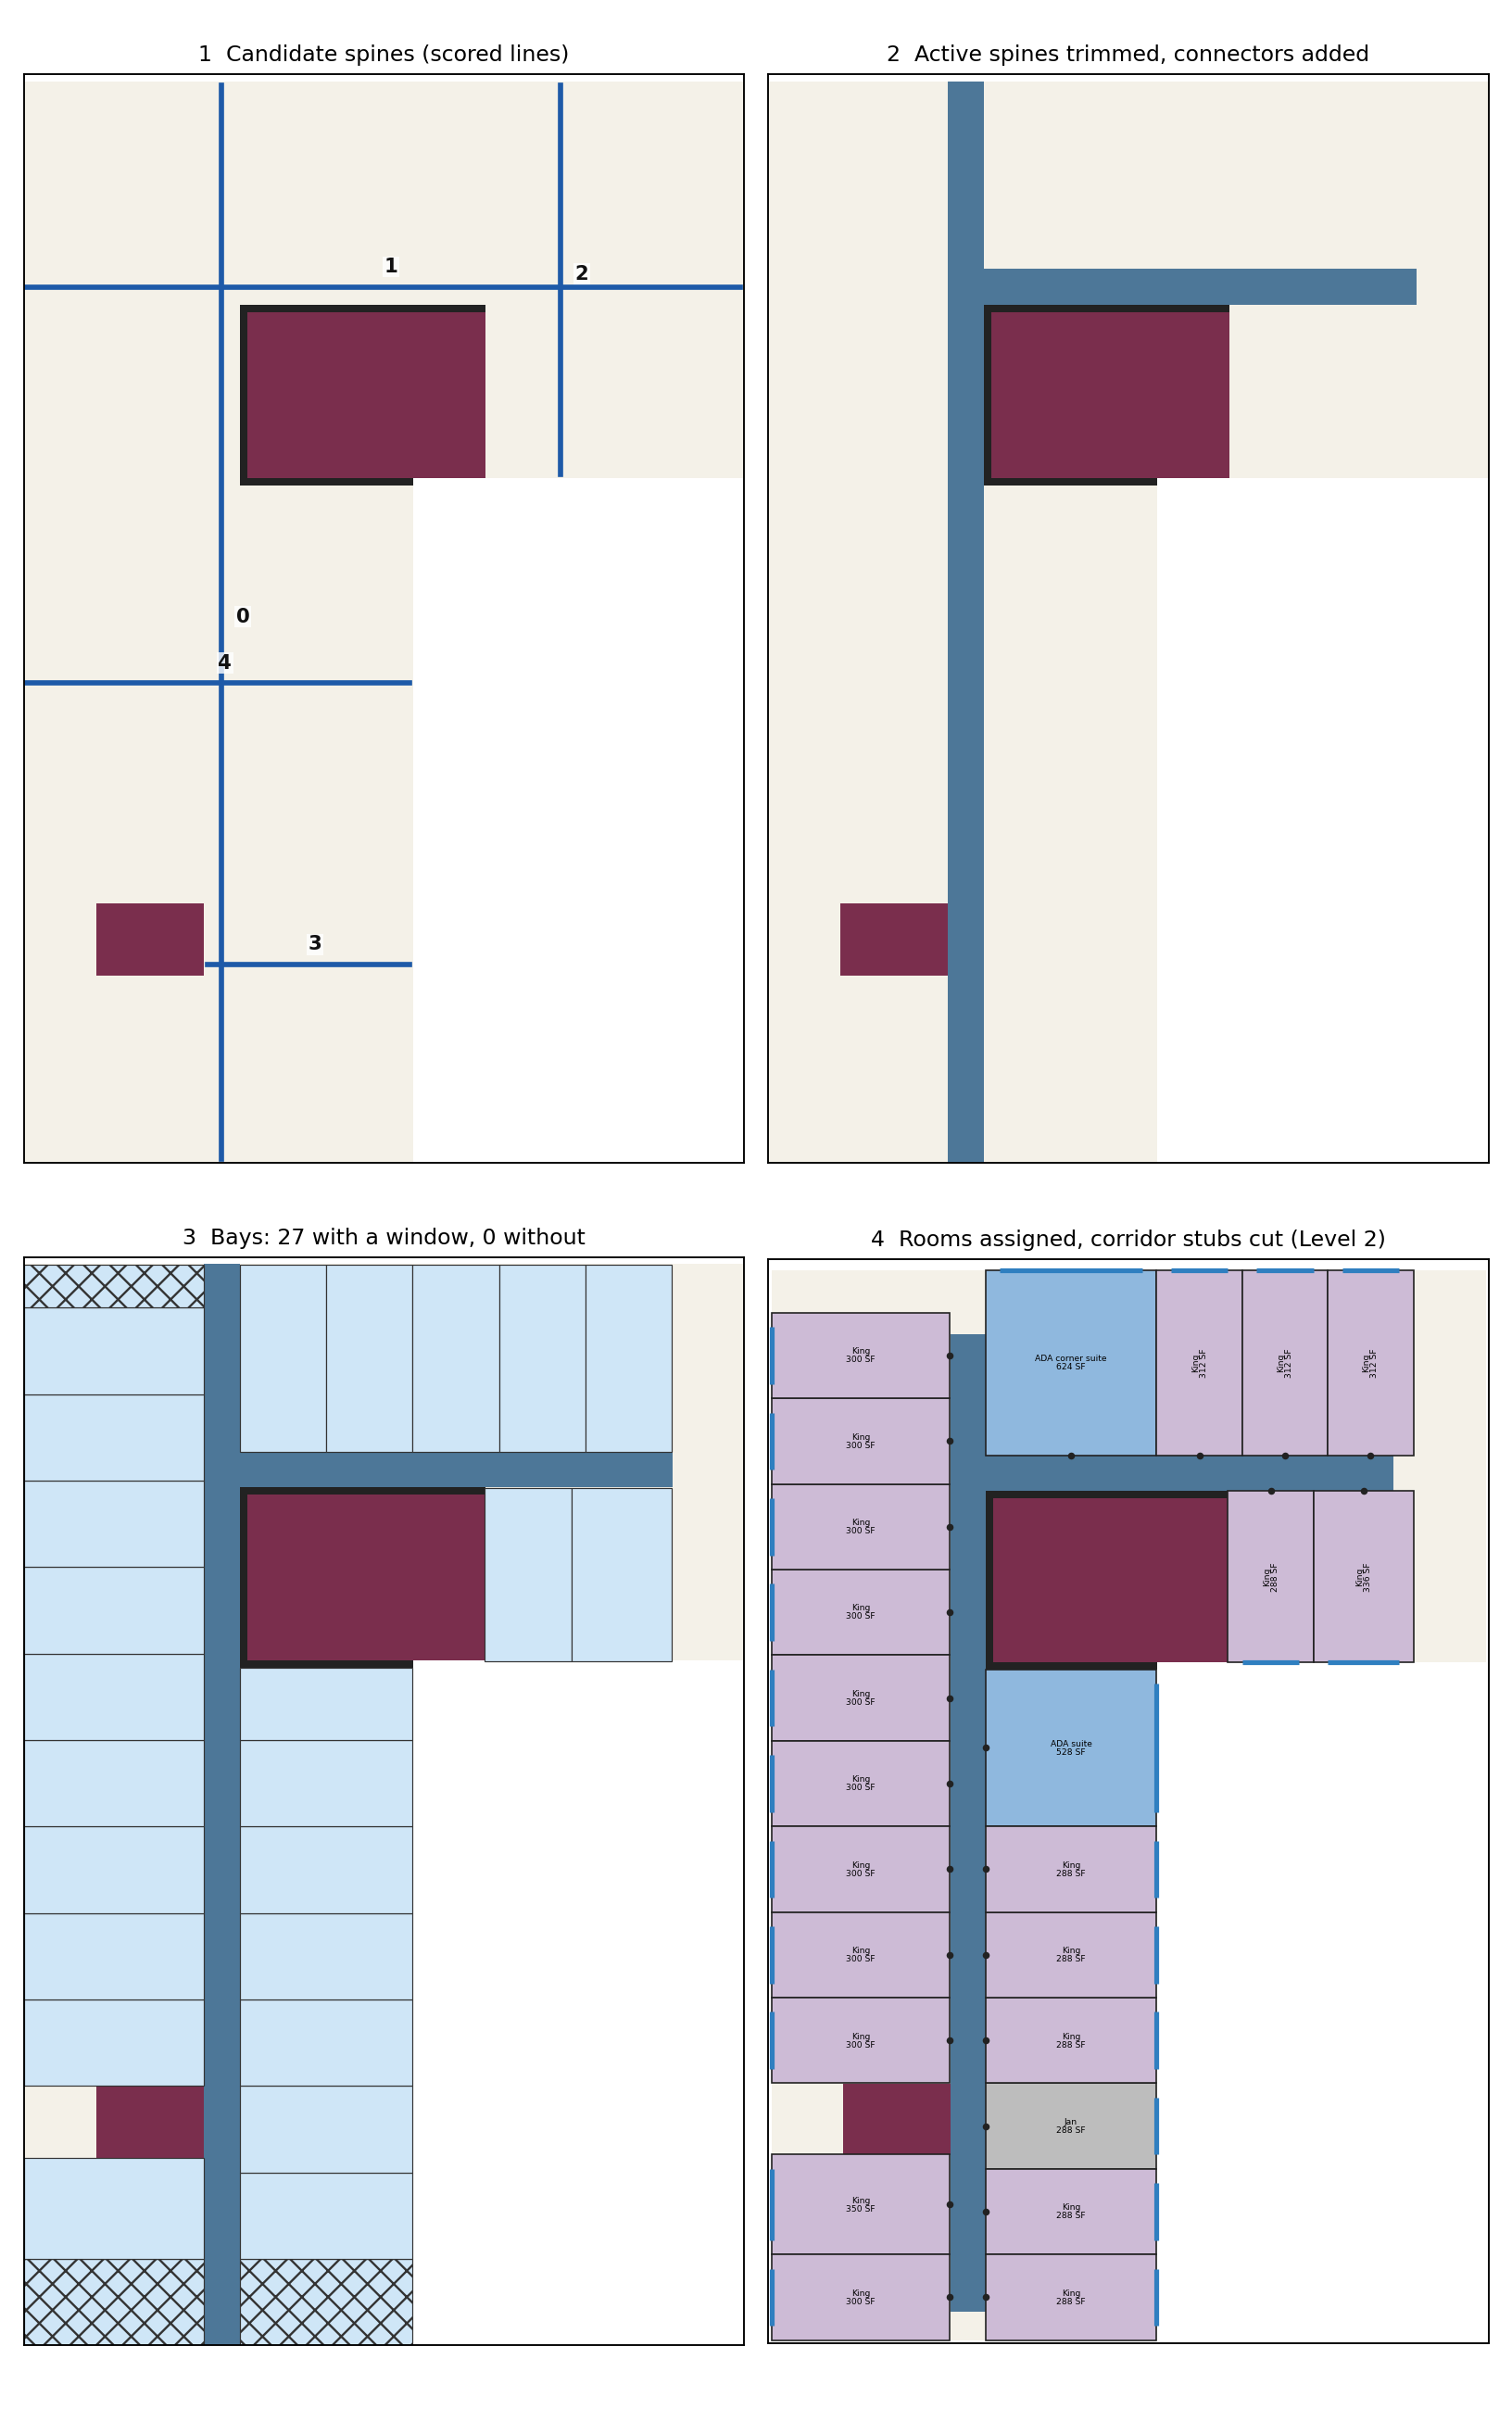
\includegraphics[width=\linewidth,height=0.86\textheight,keepaspectratio]{decoder_steps.png}\caption{The decoder on the example genome. 1: candidate spines (solid: switched on in this genome). 2: the spines that keep bays of their own, trimmed (blue), with connectors (orange, none needed here). 3: bays (light blue: with a window; hatched: corner). 4: rooms assigned.}\end{figure}

\subsection{The decoder as pseudo-code}
\begin{algorithm}[H]
\caption{Architectural decoder}
\begin{algorithmic}[1]
\Require site, program, genome $g$
\State compute $M$, $D$, $D_{\min}$, $D_{\max}$ and the candidate spines \Comment{once per site and program}
\State $S \gets$ candidates whose on/off gene $\ge 0.12$, trimmed and shifted by their genes
\State build bays along $S$; cut each spine to its own bays; drop spines with none
\State corridor $\gets S$ joined to each other and to every core by L-shaped connectors
\State bays $\gets$ window bays of all corridor sides, then windowless bays in the space left
\For{each room, in decreasing order of $0.06 \cdot \text{priority} + \text{key}$}
  \State $k \gets$ bays this room needs
  \State take the allowed run of $k$ free bays with the highest score $\sigma$; if there is none, the room is unplaced
\EndFor
\State cut each spine back to the doors and junctions it serves
\State measure exit travel and the dead end along the corridor
\State \Return layout
\end{algorithmic}
\end{algorithm}
Every genome decodes to a valid plan: corridors are straight, rooms are perpendicular to them, nothing overlaps and
every room has a door on the corridor. The search can no longer produce nonsense; it can only choose between plans.


\section{The fitness: one number for a layout}\label{sec:fitness}
The fitness contains no language model. It is arithmetic on the layout's geometry, so the same layout always gets the
same score.

\subsection{Ten objectives}
Each objective $f_k$ is scaled to lie between 0 (worst) and 1 (best):
\begingroup\footnotesize
\begin{align*}
f_{\text{place}} &= \frac{\sum_{i\ \text{placed}} p_i \min(a_i, \bar a_i)}{\sum_{i} p_i \bar a_i}, &
f_{\text{day}} &= \frac{\#\{\text{rooms needing a window that have one}\}}{\#\{\text{rooms needing a window}\}}, \\
f_{\text{eff}} &= \operatorname{clip}\!\Big(1 - \frac{\rho}{0.30}\Big), &
f_{\text{egress}} &= 1 - \tfrac12 \min\!\Big(1, \frac{(T - T_{\max})^+}{T_{\max}}\Big) - \tfrac12 \min\!\Big(1, \frac{(E - E_{\max})^+}{E_{\max}}\Big), \\
f_{\text{ada}} &= \min\!\Big(1, \frac{n_{\text{ADA}}}{n_{224.2}}\Big)\cdot\min\!\Big(1, \frac{\text{floors with ADA}}{\text{target}}\Big), &
f_{\text{core}} &= \operatorname{mean}_i \Big(1 - \frac{\min(\delta_i, 120)}{120}\Big), \\
f_{\text{adj}} &= \frac{\sum_j \omega_j \max\big(0,\ 1 - (\Delta_j - m_j)^+/m_j\big)}{\sum_j \omega_j}, &
f_{\text{corner}} &= \frac{\#\{\text{corner rooms on a corner}\}}{\#\{\text{corner rooms}\}}, \\
f_{\text{bal}} &= \operatorname{clip}\!\Big(1 - \frac{\operatorname{sd}(K_\ell)}{\operatorname{mean}(K_\ell)}\Big), &
f_{\text{comp}} &= \operatorname{clip}\!\Big(\frac{2 S_{\text{shared}}}{0.6\, P_{\text{rooms}}}\Big).
\end{align*}
\endgroup
Here $p_i$ is a room's priority, $a_i$ its drawn area and $\bar a_i$ its nominal area; $\rho$ is the corridor's share of
the placeable area; $T$ and $E$ are the exit travel and dead end of Section~\ref{sec:decoder}, with limits
$T_{\max} = 250$\,ft and $E_{\max} = 50$\,ft read from RNGD's IBC rule file; $n_{224.2}$ is the number of
accessible rooms required by ADA Table 224.2; $\delta_i$ is the door-to-core distance of a room that should be near a
core; $\Delta_j$ is the distance between the two rooms of a required adjacency and $m_j$ the distance allowed;
$K_\ell$ is the number of keys on guest floor $\ell$; $S_{\text{shared}}$ is the total length of walls shared by two
rooms and $P_{\text{rooms}}$ the total room perimeter. $(x)^+$ means $\max(0, x)$, and clip limits a value to $[0, 1]$.
An objective with nothing to measure (no required adjacency, no corner room) is 1.

\subsection{The weighted sum and the exit penalty}
\[ F = \frac{\sum_k w_k f_k}{\sum_k w_k} \; - \; \tfrac12 \max\!\big(0,\ \min(n_c, 2) - c\big), \]
where $n_c$ is the number of cores on the plate and $c$ the number the corridor reaches. A layout whose corridor
misses a required exit loses half the scale, so it can never beat one that reaches both.

\begin{example}{fitness of the example layout, term by term}
\begin{center}\centering\small
\begin{tabular}{@{}l p{6.2cm} r r r r@{}}
\toprule
\textbf{Term} & \textbf{Meaning} & \textbf{$w_k$} & \textbf{$f_k$} & \textbf{$w_k f_k$} & \textbf{Reference $f_k$} \\ \midrule
$f_{\text{place}}$ & share of the program placed (priority weighted) & 0.30 & 0.9691 & 0.2907 & 0.8911 \\
$f_{\text{day}}$ & rooms that need a window have an exterior wall & 0.14 & 1.0000 & 0.1400 & 0.8793 \\
$f_{\text{eff}}$ & corridor area kept low & 0.10 & 0.6646 & 0.0665 & 0.4952 \\
$f_{\text{egress}}$ & exit travel and dead-end corridor within IBC limits & 0.12 & 1.0000 & 0.1200 & 1.0000 \\
$f_{\text{ada}}$ & ADA mobility rooms: count (Table 224.2) and spread over floors & 0.08 & 1.0000 & 0.0800 & 1.0000 \\
$f_{\text{core}}$ & service and ADA rooms open close to a core/elevator & 0.07 & 0.9683 & 0.0678 & 0.9164 \\
$f_{\text{adj}}$ & required room adjacencies met & 0.07 & 1.0000 & 0.0700 & 1.0000 \\
$f_{\text{corner}}$ & suites on corners & 0.03 & 1.0000 & 0.0300 & 1.0000 \\
$f_{\text{bal}}$ & keys spread evenly over floors & 0.05 & 1.0000 & 0.0500 & 0.9512 \\
$f_{\text{comp}}$ & rooms share walls (compact, prefab-friendly) & 0.04 & 0.8636 & 0.0345 & 0.7036 \\
\midrule \textbf{Sum} &  & 1.00 &  & \textbf{0.9495} & \textbf{0.8798} \\
\bottomrule
\end{tabular}
\end{center}
\begin{itemize}
\item \textbf{Placement.} All 72 of 72 rooms are placed, yet $f_{\text{place}} = 0.969$, not 1. Credit is
capped at the nominal area, and a few rooms are drawn slightly smaller than nominal (the hard rule allows down to
85\%).
\item \textbf{Efficiency.} The corridor is 970\,SF of 9,640\,SF placeable, $\rho = 0.1006$, so
$f_{\text{eff}} = 1 - 0.1006/0.30 = 0.665$.
\item \textbf{Egress.} $T = 50.1$\,ft $\le 250$ and $E = 24.7$\,ft $\le 50$, so nothing is subtracted:
$f_{\text{egress}} = 1$. If the dead end were 74\,ft instead, the term would be
$1 - \tfrac12 \times (74 - 50)/50 = 0.76$.
\item \textbf{ADA.} 69 keys require 4 accessible rooms (Table 224.2). The layout has 6,
on 3 floors, so $f_{\text{ada}} = 1$.
\item \textbf{Core access.} The 9 rooms that should be near a core have their doors 3.8\,ft from one
on average.
\item \textbf{Balance.} Keys per floor are 23, 23, 23: standard deviation 0.00, so $f_{\text{bal}} = 1.000$.
\item \textbf{Compactness.} Shared walls total 1,413\,ft and room perimeters 5,454\,ft:
$2 \times 1,413 / 5,454 / 0.6 = 0.864$.
\item \textbf{Exit penalty.} The corridor reaches 2 of 2 cores, so the penalty is 0.
\end{itemize}
The weights sum to 1.00, so $F = 0.9495$. The last column scores the reference GA's layout for the same site with
the same formulas: it loses most on placement, daylight and corridor efficiency.
\end{example}

\begin{example}{what the exit penalty does}
Take a layout with $F = 0.90$ before the penalty on a plate with two cores. If its corridor reaches only one of them,
$F = 0.90 - \tfrac12 (2 - 1) = 0.40$. Any layout that connects both exits scores higher, however poor it is otherwise.
\end{example}


\section{Algorithm C: the updated genetic algorithm}\label{sec:ga}
The updated GA uses the architectural decoder and adds a short local search to every generation, which makes it a
\emph{memetic} algorithm. It is seeded, so a run can be repeated exactly.

\subsection{One generation}
\begin{algorithm}[H]
\caption{Updated (memetic) GA}
\begin{algorithmic}[1]
\Require population size $P$, generations $G$, seed
\State population $\gets$ six spine-set seeds $+$ three random genomes $+$ random genomes up to $P$
\For{$t = 1$ \textbf{to} $G$}
  \State $\sigma_t \gets \sigma_{\text{start}} + (\sigma_{\text{end}} - \sigma_{\text{start}})\,\frac{t-1}{G-1}$ \Comment{mutation strength falls}
  \State next $\gets$ the 2 best individuals \Comment{elitism}
  \State improve the best one by 4 trial mutations of strength $\sigma_t/2$, keeping each one only if it is better \Comment{local search}
  \If{the population's fitness values are nearly equal (standard deviation $< 0.01$)}
    \State add 2 random genomes \Comment{immigrants}
  \EndIf
  \While{next has fewer than $P$ individuals}
    \State pick two parents, each the best of 3 individuals drawn at random \Comment{tournament selection}
    \State child $\gets$ crossover(parents) with probability 0.9, otherwise a copy of the first parent
    \State child $\gets$ mutate(child, $\sigma_t$); decode and score it; add it to next
  \EndWhile
  \State population $\gets$ next
\EndFor
\State \Return the best individual
\end{algorithmic}
\end{algorithm}

\subsection{The starting population}
A purely random start wastes generations rediscovering the obvious. Six seeds therefore switch on fixed sets of
spines: all of them, the best one, the best two, the best three, the best four, and every second one. Three more
genomes are random, and the rest of the population is filled with random genomes in which each spine is off with
probability 0.4.

\subsection{Selection}
To pick a parent, 3 individuals are drawn at random and the fittest wins. Better individuals are picked more
often, but a weaker one still wins when it happens to be drawn with even weaker ones, which keeps variety in the
population.

\subsection{Crossover}
\begin{itemize}
\item For each of the eleven gene blocks (ten spines and the connector block) a coin decides which parent it comes
from. A spine is inherited whole: its trims, its shift and its on/off gene stay together.
\item For each room's order key another coin decides.
\end{itemize}
\begin{example}{a crossover that helps}
\begin{itemize}
\item Parent 1: spines \{0, 1, 2\}, 53 rooms, $F = 0.894$.
\item Parent 2: spines \{0, 2, 4\}, 66 rooms, $F = 0.872$.
\item The child takes spine blocks \{0, 2, 3, 4\} and the connector genes and 29 of its 72 order keys from parent 2, the rest from parent 1.
\item Child (before mutation): spines \{0, 1, 2, 4\}, 72 rooms, $F = 0.949$.
\end{itemize}
The child is better than both parents: the mix happened to combine a good corridor set with a workable room order.
\end{example}
\begin{example}{a crossover that hurts}
\begin{itemize}
\item Parent 1: spines \{0, 1, 2, 3, 4\}, 63 rooms, $F = 0.902$.
\item Parent 2: spines \{0, 2, 3, 4\}, 52 rooms, $F = 0.850$.
\item The child takes spine blocks \{1, 3\} and 34 of its 72 order keys from parent 2, the rest from parent 1.
\item Child (before mutation): spines \{0, 2, 3, 4\}, 51 rooms, $F = 0.793$.
\end{itemize}
The child is worse than both parents. Each parent's room order was tuned to its own corridors; put on a different corridor set, the order no longer fits.
\end{example}

\begin{example}{what crossover achieved over a whole run}
I logged every crossover in the example run and scored each child \emph{before} mutation, next to its two parents
(540 crossovers):
\begin{itemize}
\item 43 children (8\%) were better than their better parent;
\item 126 (23\%) scored the same as their better parent;
\item 220 (41\%) fell between the two parents;
\item 151 (28\%) were worse than both.
\end{itemize}
On average the better parent scored 0.9486 and the child 0.9451. Crossover sometimes produces the jump that matters
(the first example above), but most of the time it does not improve on what the parents already had. This matches
the review comment that splicing two plans seldom makes architectural sense, and it is why the default search
(Section~\ref{sec:sys}) does without it.
\end{example}

\subsection{Mutation}
A child is changed in four ways:
\begin{itemize}
\item \textbf{Gaussian noise} of standard deviation $\sigma_t$ on about 30\% of the 44 corridor genes;
\item \textbf{spine toggles}: each of the eleven blocks flips its on/off gene with probability 0.08;
\item \textbf{key swaps}: with probability 0.45, 3 pairs of rooms exchange their order keys;
\item \textbf{Gaussian noise} on about 10\% of the order keys.
\end{itemize}
All genes are then clipped to $[0, 1]$. The strength $\sigma_t$ falls linearly from 0.15 in the first generation to
0.03 in the last: wide exploration early, fine adjustment late.

\begin{example}{one mutation at full strength}
Mutating the final best genome once with $\sigma = 0.15$ changed 13 of 44 corridor genes and
12 of 72 order keys. The active spines changed from \{0, 1, 2, 4\} to \{1, 2, 4\}, and the fitness went from 0.954 to
0.792. One toggled spine is enough to change the plan completely, which is why the best individual is always carried
over unchanged (elitism) and why mutation gets weaker over the run.
\end{example}

\subsection{The example run}
\begin{table}[H]\centering\small\caption{The GA on the running example (population 24, 30 generations, seed 7).}\label{tab:ga}
\begin{tabular}{@{}r r r r r r@{}}
\toprule
\textbf{Generation} & \textbf{$\sigma_t$} & \textbf{Best $F$} & \textbf{Mean $F$ of population} & \textbf{Rooms (best)} & \textbf{Layouts evaluated} \\ \midrule
1 & 0.150 & 0.9493 & 0.9049 & 72 & 50 \\
2 & 0.146 & 0.9493 & 0.9032 & 72 & 76 \\
3 & 0.142 & 0.9493 & 0.9261 & 72 & 102 \\
5 & 0.133 & 0.9493 & 0.9296 & 72 & 154 \\
10 & 0.113 & 0.9495 & 0.9246 & 72 & 284 \\
15 & 0.092 & 0.9503 & 0.9275 & 72 & 414 \\
20 & 0.071 & 0.9506 & 0.8984 & 72 & 544 \\
25 & 0.051 & 0.9513 & 0.9325 & 72 & 674 \\
30 & 0.030 & 0.9536 & 0.9221 & 72 & 804 \\
\bottomrule
\end{tabular}
\end{table}
The run evaluated 804 layouts: $P = 24$ to start, then in each of 30 generations
$P - 2 = 22$ children and 4 local-search trials, $24 + 30 \times (22 + 4) = 804$.
It ended with 72 of 72 rooms and $F = 0.9536$. The best layout was already close after the first
generation (the seeds do most of the work); the rest of the run adds small gains.


\section{Algorithm D: the systematic search (default)}\label{sec:sys}
With the architectural decoder the important decision is small: which of at most ten spines are on. A space that
small can be searched in an orderly way, with no population and no crossover. The search has three stages and a fixed
budget of $P \times G$ layouts, the same as the GA's.

\subsection{Stage 1: enumerate the spine sets}
With $m$ candidate spines the first stage tries
\begin{itemize}
\item all spines switched on, and
\item every set of one, two, three or four of the seven best spines,
\end{itemize}
each with no trim, no shift and all order keys at 0.5 (rooms in priority order). That is
\[ 1 + \sum_{k=1}^{4} \binom{\min(m,7)}{k} \;\le\; 1 + 7 + 21 + 35 + 35 = 99 \text{ layouts.} \]

\begin{example}{stage 1 on \code{fp1}}
The plate has $m = 5$ candidates, so stage 1 evaluates $1 + 5 + 10 + 10 + 5 = 31$ spine sets.
\begin{center}\centering\small
\begin{tabular}{@{}l r r@{}}
\toprule
\textbf{Spines switched on} & \textbf{Rooms placed} & \textbf{Fitness $F$} \\ \midrule
\{0, 1, 2, 3, 4\} & 72 & 0.9460 \\
\{0, 1\} & 72 & 0.9460 \\
\{0, 1, 2\} & 72 & 0.9460 \\
\{0, 1, 3\} & 72 & 0.9460 \\
\{0, 1, 4\} & 72 & 0.9460 \\
\{0, 1, 2, 3\} & 72 & 0.9460 \\
\ldots &  &  \\
\{2, 4\} & 15 & 0.7703 \\
\{3, 4\} & 9 & 0.7478 \\
\{4\} & 6 & 0.7267 \\
\bottomrule
\end{tabular}
\end{center}
Fitness ranges from 0.727 to 0.946. Two things stand out:
\begin{itemize}
\item \textbf{The corridor set decides almost everything.} Spine 4 alone places 6 rooms; any set containing
spines 0 and 1 places all 72.
\item \textbf{Different sets can give the same plan.} The best sets all contain spines 0 and 1 and have the same
fitness, because the decoder drops the extra spines when they get no bays of their own (Step 4 of
Section~\ref{sec:decoder}).
\end{itemize}
\end{example}

\subsection{Stage 2: pattern search from the three best}
The three best \emph{distinct} layouts of stage 1 become starting points. For each one the search generates its
\emph{neighbours}, the layouts one small move away:
\begin{itemize}
\item switch one spine on or off (10 moves);
\item for each active spine: trim the low end, trim the high end, shift it one way, shift it the other (4 moves each);
\item redraw the connector elbows (1 move);
\item move a few rooms earlier or later in the assignment order (4 moves, about one room in twelve each).
\end{itemize}
The neighbours are evaluated in a seeded random order, and the \textbf{first one that is better is accepted}
($F' > F + 10^{-6}$). The search then continues from the new layout. When no neighbour is better, that start is a
\emph{local optimum} and is left alone.

\begin{example}{one descent, move by move}
Starting from the best stage-1 layout (spines \{0, 1, 2, 3, 4\}) and applying the rule above:
\begin{center}\centering\small
\begin{tabular}{@{}r r p{6.2cm} r r r@{}}
\toprule
\textbf{Step} & \textbf{Neighbours tried} & \textbf{Accepted move} & \textbf{$F$ before} & \textbf{$F$ after} & \textbf{Rooms} \\ \midrule
1 & 9 & 6 rooms moved later in the order & 0.9460 & 0.9461 & 72 \\
2 & 5 & 6 rooms moved earlier in the order & 0.9461 & 0.9474 & 72 \\
3 & 35 & no neighbour is better: local optimum & 0.9474 & 0.9474 & 72 \\
\bottomrule
\end{tabular}
\end{center}
The descent tried 49 neighbours in total. With 5 active spines a neighbourhood has
$10 + 4 \times 5 + 1 + 4 = 35$ moves; the last row shows all of them tried without success.
\end{example}

\subsection{Stage 3: iterated local search}
If all three starts are local optima and budget remains, the search \emph{kicks} the best layout: it applies two
random moves at once, which is enough to leave the local optimum. It then descends again with the same pattern search
and keeps the result only if it beats the best layout so far. This repeats until the budget is used.

\subsection{The whole run on the example}
\begin{example}{every improvement after stage 1}
The real run made 720 decoder calls (695 distinct layouts; a genome seen before is not decoded again).
After the 31 layouts of stage 1, the best fitness rose 3 times:
\begin{center}\centering\small
\begin{tabular}{@{}r p{7.5cm} r r@{}}
\toprule
\textbf{Decoder call} & \textbf{Move that produced it} & \textbf{$F$ of its parent} & \textbf{$F$ after} \\ \midrule
41 & 6 rooms moved earlier in the order & 0.9460 & 0.9475 \\
67 & spine 1 trimmed at its high end & 0.9475 & 0.9492 \\
97 & spine 1 trimmed at its high end & 0.9475 & 0.9495 \\
\bottomrule
\end{tabular}
\end{center}
The run ended with 72 of 72 rooms and $F = 0.9495$. A second run with the same inputs returned exactly the
same genome and fitness: yes.
\end{example}
\begin{figure}[H]\centering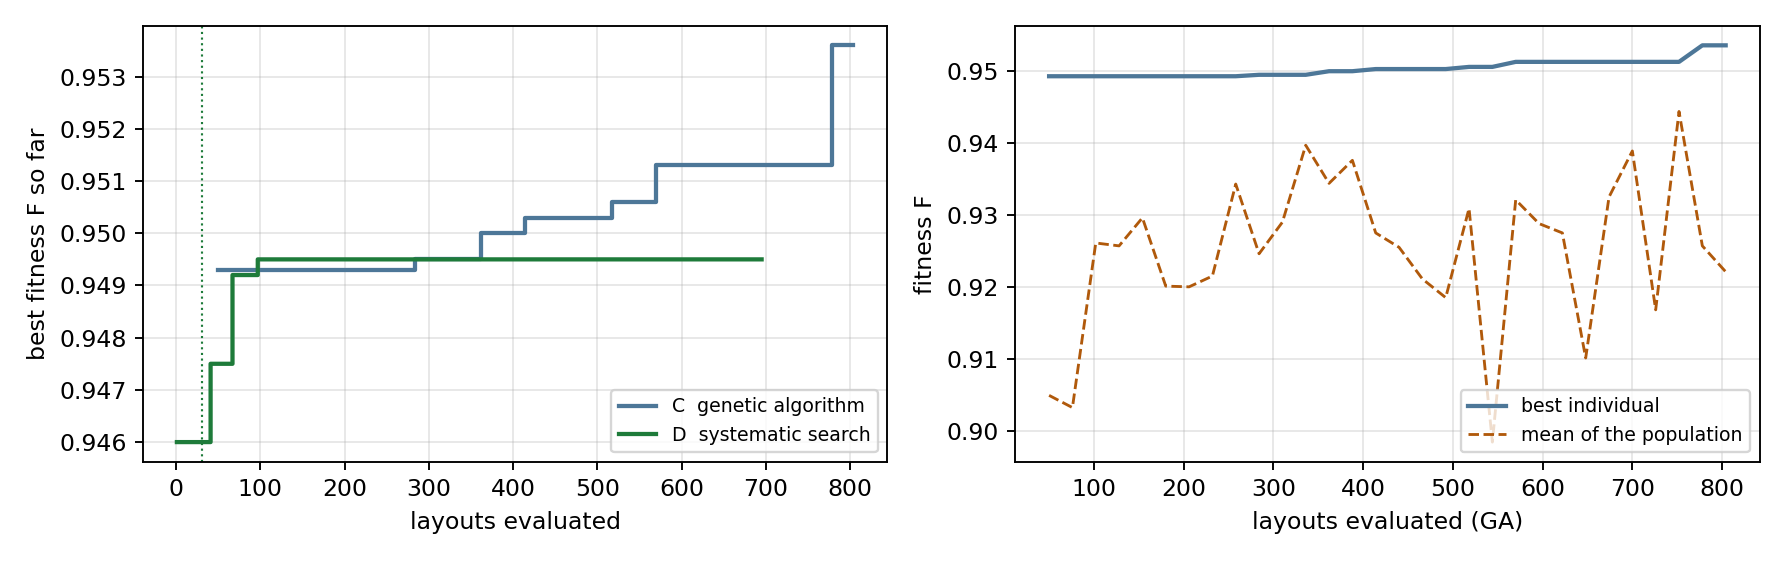
\includegraphics[width=\linewidth,height=0.28\textheight,keepaspectratio]{convergence.png}\caption{The two searches on the running example, same decoder and same budget. Left: best fitness so far against layouts evaluated; the dotted line marks the end of stage 1 of the systematic search. Right: the GA's best individual and the mean fitness of its population, which stays well below the best because mutation keeps breaking good plans.}\end{figure}

\begin{algorithm}[H]
\caption{Systematic search}
\begin{algorithmic}[1]
\Require budget $B = P \times G$ layouts, seed
\State evaluate every spine set of stage 1 \Comment{at most 99 layouts}
\State starts $\gets$ the three best distinct layouts
\While{budget remains and some start is not a local optimum}
  \For{each start $x$ that is not a local optimum}
    \State evaluate the neighbours of $x$ in seeded random order; move $x$ to the first better one
    \State if none is better, mark $x$ as a local optimum
  \EndFor
\EndWhile
\While{budget remains} \Comment{iterated local search}
  \State $y \gets$ best layout so far, changed by two random moves
  \State descend from $y$ by the same pattern search
  \State if $y$ is now better than the best layout, it becomes the best
\EndWhile
\State \Return the best layout
\end{algorithmic}
\end{algorithm}


\section{The algorithms side by side}
\begin{table}[H]\centering\small\caption{All four algorithms on the three sites, same program, same fitness (budget 24 $\times$ 30 for B, C and D, seed 7). ``No window'' counts guest rooms without a facade wall.}\label{tab:comp}
\begin{tabular}{@{}l l r r r r r r@{}}
\toprule
\textbf{Site} & \textbf{Algorithm} & \textbf{Rooms} & \textbf{No window} & \textbf{$F$} & \textbf{Evaluated} & \textbf{Time} & \textbf{Checks} \\ \midrule
fp1 & A reference GA & 61/72 & 7 & 0.880 & 500 gen. & n/a & 6/6 \\
 & B first attempt & 53/72 & 3 & 0.880 & 804 & 119\,s & 5/6 \\
 & C updated GA & 72/72 & 0 & 0.954 & 804 & 24\,s & 6/6 \\
 & D systematic & 72/72 & 0 & 0.950 & 695 & 20\,s & 6/6 \\ \midrule
fp2 & A reference GA & 53/72 & 8 & 0.860 & 500 gen. & n/a & 6/6 \\
 & B first attempt & 60/72 & 8 & 0.893 & 804 & 102\,s & 6/6 \\
 & C updated GA & 62/72 & 0 & 0.908 & 804 & 22\,s & 6/6 \\
 & D systematic & 60/72 & 0 & 0.904 & 637 & 17\,s & 6/6 \\ \midrule
fp3 & A reference GA & 57/72 & 9 & 0.851 & 500 gen. & n/a & 6/6 \\
 & B first attempt & 61/72 & 3 & 0.894 & 804 & 115\,s & 6/6 \\
 & C updated GA & 63/72 & 0 & 0.921 & 804 & 26\,s & 6/6 \\
 & D systematic & 60/72 & 0 & 0.911 & 683 & 21\,s & 6/6 \\
\bottomrule
\end{tabular}
\end{table}
\begin{itemize}
\item \textbf{The decoder matters more than the search.} B has a better search and scoring than A but the same kind
of decoder, and its plans keep the windowless rooms. C and D share the new decoder and neither has any.
\item \textbf{GA or systematic?} At the same budget the GA (C) finishes slightly ahead on fitness: 0.928 against
0.922 on average, 197 rooms against 192. Its random order keys and crossover occasionally find a room order
that the move-by-move search does not reach.
\item \textbf{Why the systematic search is still the default.} It has no population size, crossover rate or mutation
schedule to tune, it explains itself (every improvement is one named move), and it gives the same answer every time.
The GA is one setting away in the Design Optimizer when the last few thousandths matter.
\end{itemize}


\section{Algorithm E: exploring hotel layouts (shape, core and floors)}\label{sec:hotel}
On the prototype's sites the plate and the cores are given. In the Hotel Schematic mode they are not: only the program
and the buildable area are. An outer loop therefore \emph{generates} plates and runs the decoder on each.

\subsection{Sizing a plate}
For $K$ keys on $F$ guest floors, let $A$ be the net room area of the busiest level. With a slack factor
$\varsigma = 1.04$, core area $A_c$ and a packing efficiency $\eta = 0.93$, the plate must offer a corridor of length
\[ R = \frac{\varsigma A + A_c}{2 D \eta}, \]
because every foot of double-loaded corridor serves $2D$ square feet of rooms. Each shape with bounding box
$a \times b$ and wing depth $W_d = 2D + w$ offers
\[ R_{\text{Bar}} = a,\quad R_{\text{L}} = R_{\text{T}} = a + b - W_d,\quad R_{\text{U}} = R_{\text{H}} = a + 2b - 2W_d,\quad
R_{\text{Courtyard}} = 2a + 2b - 4W_d . \]
For each shape the generator finds the smallest $a$ with $R_{\text{shape}}(a, \beta a) \ge R$ at aspect ratios
$\beta \in \{0.6, 1\}$, in both orientations, and clips the result to the buildable area.

\begin{example}{plates for 117 keys on 4 guest floors}
\begin{itemize}
\item Net area per level: 12,148, 10,995, 10,995, 10,995, 10,995\,SF. The busiest is Level 1 with $A = 12,148$\,SF.
\item Elevators: $\max(2, \lceil 117/75 \rceil) = 2$. The main core is 32 $\times$ 26\,ft and each
stair 14 $\times$ 26\,ft, so $A_c = 1,560$\,SF.
\item Room depth $D = 26$\,ft and corridor $w = 6$\,ft give a wing depth $W_d = 58$\,ft.
\item $R = (1.04 \times 12,148 + 1,560) / (2 \times 26 \times 0.93) = 293.5$\,ft.
\end{itemize}
A Bar needs $a = 294$\,ft, more than the 265\,ft the buildable area allows, so it is clipped to 265\,ft
(the layout then has to do with less corridor than the estimate asks for). The generator produces 41 plates for this floor count:
\begin{center}\centering\small
\begin{tabular}{@{}l c r r r c l@{}}
\toprule
\textbf{Shape} & \textbf{$a \times b$, ft} & \textbf{Corridor run, ft} & \textbf{Footprint, SF} & \textbf{Facade, ft} & \textbf{Clipped} & \textbf{Core schemes} \\ \midrule
Bar & 265 $\times$ 58 & 265 & 15,370 & 646 & yes & center, ends \\
L & 170 $\times$ 132 & 244 & 14,152 & 604 & yes & center, ends, knuckle \\
L & 220 $\times$ 132 & 294 & 17,052 & 704 & no & center, ends, knuckle \\
L & 170 $\times$ 176 & 288 & 16,704 & 692 & yes & center, ends, knuckle \\
L & 176 $\times$ 170 & 288 & 16,704 & 692 & yes & center, ends, knuckle \\
U & 170 $\times$ 112 & 278 & 16,124 & 672 & yes & center, ends, knuckle \\
U & 187 $\times$ 112 & 295 & 17,110 & 706 & no & center, ends, knuckle \\
U & 156 $\times$ 127 & 294 & 17,052 & 704 & no & center, ends, knuckle \\
T & 170 $\times$ 132 & 244 & 14,152 & 604 & yes & center, ends, knuckle \\
T & 220 $\times$ 132 & 294 & 17,052 & 704 & no & center, ends, knuckle \\
T & 170 $\times$ 176 & 288 & 16,704 & 692 & yes & center, ends, knuckle \\
T & 176 $\times$ 170 & 288 & 16,704 & 692 & yes & center, ends, knuckle \\
H & 156 $\times$ 136 & 312 & 18,096 & 740 & no & center, ends, knuckle \\
Courtyard & 156 $\times$ 156 & 392 & 22,736 & 784 & no & center, ends, knuckle \\
\bottomrule
\end{tabular}
\end{center}
\end{example}
\begin{figure}[H]\centering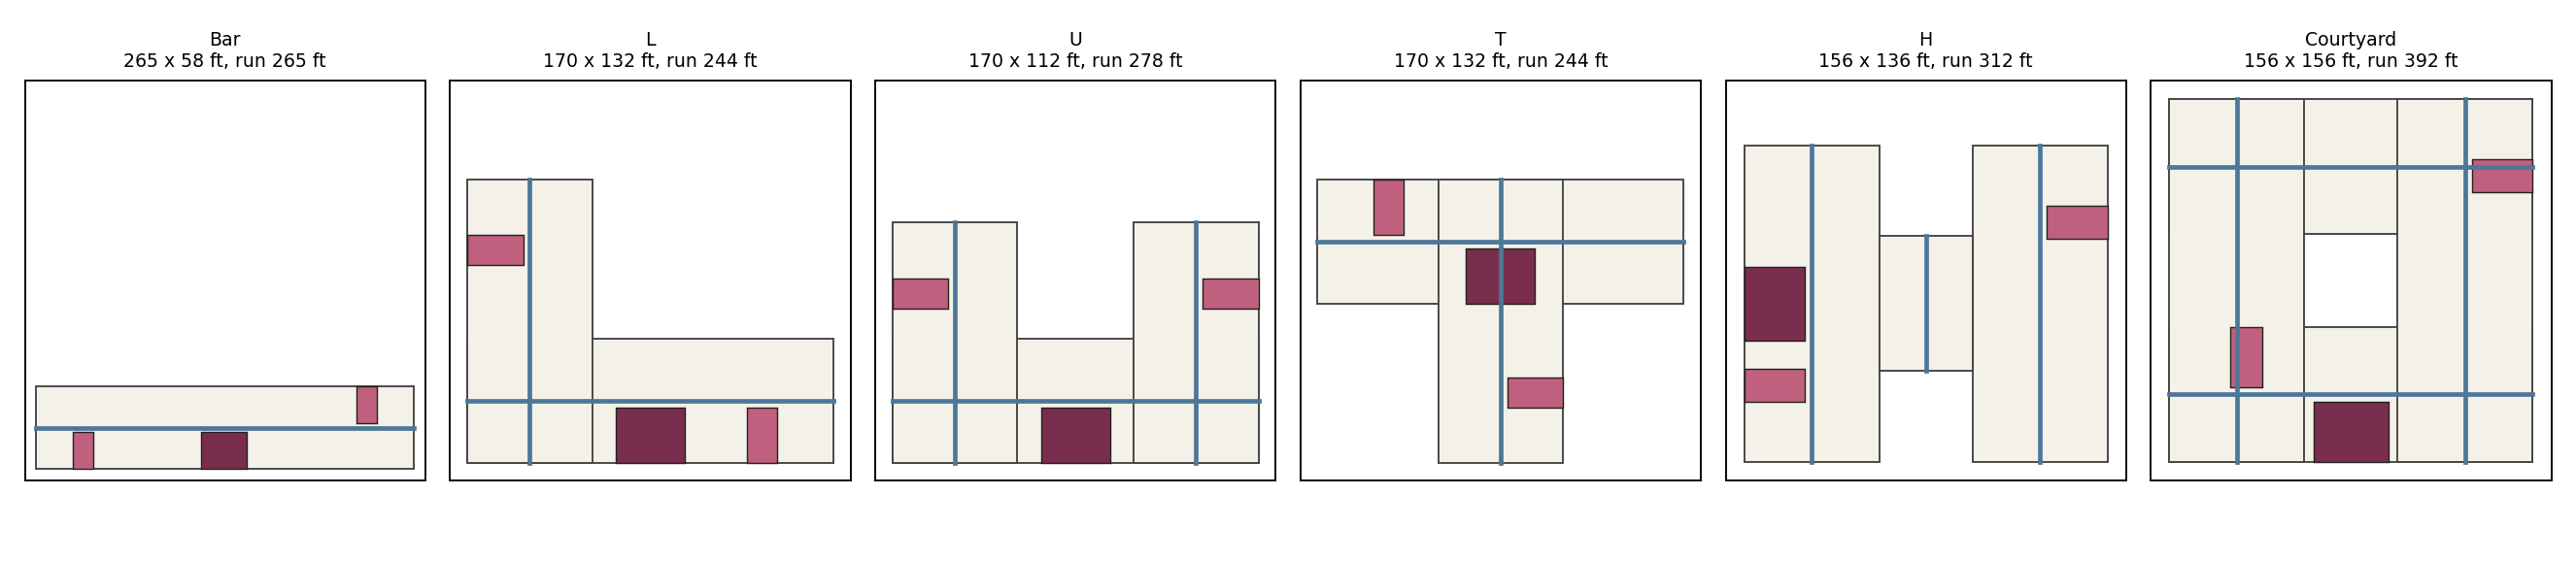
\includegraphics[width=\linewidth,height=0.26\textheight,keepaspectratio]{plates.png}\caption{One generated plate per shape with the centre-core scheme. Dark: elevator core; lighter: stairs; blue: corridor centre-lines.}\end{figure}

\subsection{Cores and stairs}
Each plate is tried with up to three core schemes:
\begin{itemize}
\item \textbf{ends}: the elevator core near one end, a stair near the other;
\item \textbf{center}: the elevator core at the middle of the longest wing, and two stairs at the pair of wing ends
that are farthest apart (which helps exit separation and keeps dead ends short);
\item \textbf{knuckle}: the elevator core where two wings meet, with stairs at the far ends.
\end{itemize}

\subsection{The three stages}
\begin{enumerate}
\item \textbf{Screen.} Every plate, for every floor count tried (the requested count, one fewer, and up to two more,
within the height limit), is decoded with 6 fixed spine sets (all spines, the best one, two, three and four,
and every second one), rooms in priority order. Plates are independent, so they run in parallel processes.
\item \textbf{Refine.} The best plate of each shape, then the next best overall up to 8 plates, are improved by
the pattern search of Section~\ref{sec:sys} for 24 evaluations each.
\item \textbf{Archive.} Every distinct layout is kept. Two layouts count as the same if they have the same plate,
floor count, rooms placed, corridor area, shared-wall length and fitness (to three decimals).
\end{enumerate}
One extra code check is added here because the floor count now varies: the number of stories (guest floors plus the
ground level) must not exceed 5.

\begin{example}{the run on the Living\,+\,Lodging program}
Buildable area 170 $\times$ 265\,ft. The exploration screened 158 plate and floor-count variants,
evaluated 1,140 layouts ($158 \times 6$ in screening plus $8 \times 24$ in
refinement) and kept 740 distinct ones in 36\,s on eight processes. Refinement gains were small:
Courtyard 156x156 $\cdot$ center core, 5 floors: 0.870 $\to$ 0.870; L 202x121 $\cdot$ ends core, 5 floors: 0.863 $\to$ 0.881; Bar 265x58 $\cdot$ center core, 5 floors: 0.863 $\to$ 0.863. The layout ranked first (next section) is Bar 265x58 $\cdot$ center core with 4 guest floors.
\end{example}

\subsection{An upper bound per floor}
Along a corridor of length $R$, both sides together offer $2R$ feet of frontage, less the frontage $c_f$ taken by the
cores. No layout can have more than
\[ K_{\text{floor}} = \Big\lfloor \frac{2R - c_f}{M} \Big\rfloor \]
keys on a typical floor.
\begin{example}{bound for the Bar 265x58 $\cdot$ center core plate}
$R = 265$\,ft, the cores take $c_f = 84$\,ft (the longer side of each of the 3 cores) and the module
is $M = 13$\,ft: $\lfloor (2 \times 265 - 84)/13 \rfloor = 34$ keys per floor, so at most
$34 \times 4 = 136$ on 4 floors, against 117 requested. The bound is loose (it ignores suites, which
take two bays, and the per-floor service rooms), but it shows at once whether a request can fit.
\end{example}


\section{Choosing among the layouts: Pareto front and TOPSIS}\label{sec:decide}
The exploration returns hundreds of layouts. Which is best depends on what the owner values: the most keys, the lowest
cost, the lowest building. That choice is kept separate from the fitness and is made in two deterministic steps over
12 criteria (fitness, keys, share of the program placed, daylight, corridor share, gross area per key, facade
per key, height, dead end, exit travel, code checks passed, compactness).

\subsection{Pareto front}
Layout $x$ \emph{dominates} layout $y$ if $x$ is at least as good as $y$ on every criterion and strictly better on at
least one. A layout that nothing dominates is on the \emph{Pareto front}. A dominated layout is never the right
choice, whatever the priorities.

\subsection{TOPSIS}
TOPSIS ranks all layouts for a given set of weights $\lambda_q$:
\begin{enumerate}
\item \textbf{Normalise} each criterion $q$ over the layouts $j$: $r_{jq} = x_{jq} / \sqrt{\sum_j x_{jq}^2}$.
\item \textbf{Weight}: $v_{jq} = \dfrac{\lambda_q}{\sum_q \lambda_q}\, r_{jq}$.
\item Find the \textbf{ideal} $v_q^+$ (the best value of each criterion over all layouts) and the \textbf{worst}
$v_q^-$. ``Best'' is the largest value for a criterion to maximise and the smallest for one to minimise.
\item Measure each layout's \textbf{distance} to both: $d_j^{\pm} = \sqrt{\sum_q (v_{jq} - v_q^{\pm})^2}$.
\item The \textbf{closeness} $C_j = \dfrac{d_j^-}{d_j^+ + d_j^-}$ lies between 0 and 1. The layout with the largest
$C_j$ is ranked first.
\end{enumerate}

\begin{example}{four real layouts, three criteria}
To keep the arithmetic visible, take four layouts from the hotel run and only three of the criteria, with the weights
of the Balanced preset: Fitness (all objectives) (maximise, $\lambda = 3$), Gross SF per key (minimise, $\lambda = 1$) and Dead-end corridor
(minimise, $\lambda = 1$).
\begin{center}\centering\footnotesize
\begin{tabular}{@{}l l r r r r l@{}}
\toprule
\textbf{} & \textbf{Layout} & \textbf{Floors} & \textbf{Fitness} & \textbf{SF per key} & \textbf{Dead end, ft} & \textbf{On these three criteria} \\ \midrule
A & Bar 265x58 $\cdot$ center core & 4 & 0.859 & 657 & 24.1 & on the front \\
B & L 220x132 $\cdot$ knuckle core & 4 & 0.849 & 729 & 26.1 & dominated by A \\
C & Courtyard 156x156 $\cdot$ ends core & 4 & 0.845 & 972 & 28.1 & dominated by A \\
D & Bar 265x58 $\cdot$ center core & 5 & 0.863 & 788 & 24.1 & on the front \\
\bottomrule
\end{tabular}
\end{center}
Layout B is dominated by A: A has higher fitness (0.859 against 0.849), less area per key (657 against 729\,SF) and a dead end that is no longer (24.1 against 26.1\,ft). Layouts A and D are both on the front: D has the higher fitness (0.863 against 0.859) but needs more area per key (788 against 657\,SF), so neither beats the other on everything.

Normalisers $\sqrt{\sum_j x_{jq}^2}$ are 1.708, 1,589.9 and 51.3; the weights become 0.6, 0.2, 0.2
(each $\lambda_q$ divided by 5).
\begin{center}\centering\small
\begin{tabular}{@{}l r r r r r r r r r@{}}
\toprule
\textbf{} & \textbf{$r_1$} & \textbf{$r_2$} & \textbf{$r_3$} & \textbf{$v_1$} & \textbf{$v_2$} & \textbf{$v_3$} & \textbf{$d^+$} & \textbf{$d^-$} & \textbf{$C$} \\ \midrule
A & 0.5030 & 0.4131 & 0.4697 & 0.3018 & 0.0826 & 0.0939 & 0.0012 & 0.0428 & \textbf{0.974} \\
B & 0.4972 & 0.4583 & 0.5087 & 0.2983 & 0.0917 & 0.1017 & 0.0128 & 0.0316 & \textbf{0.711} \\
C & 0.4947 & 0.6111 & 0.5477 & 0.2968 & 0.1222 & 0.1095 & 0.0430 & 0.0000 & \textbf{0.000} \\
D & 0.5050 & 0.4958 & 0.4697 & 0.3030 & 0.0992 & 0.0939 & 0.0165 & 0.0285 & \textbf{0.633} \\
\bottomrule
\end{tabular}
\end{center}
The ideal point is $(0.3030, 0.0826, 0.0939)$ and the worst $(0.2968, 0.1222, 0.1095)$. For layout A,
$C = 0.0428 / (0.0012 + 0.0428) = 0.974$. The ranking is A $>$ B $>$ D $>$ C.

With all 12 criteria and all 740 layouts the same procedure produces the ranking shown in the app. The
Pareto flags can differ from this small example, because a layout dominated on three criteria may be the best on a
fourth.
\end{example}

\subsection{Presets}
The app offers five weight presets (Balanced, Most keys, Lowest cost, Guest experience, Low-rise) and sliders. Changing
the weights re-ranks the stored layouts instantly; nothing is searched again. In the hotel run the Balanced preset
ranks Bar 265x58 $\cdot$ center core first, while Most keys ranks Courtyard 156x156 $\cdot$ center core first.


\section{How good can any algorithm be? Two upper bounds}
Before judging a search it helps to know what is possible at all. Two bounds hold for every layout.

\textbf{Area.} A corridor of width $w$ serves at most two room depths, so at least $w/(2D + w)$ of the used floor is
corridor. With $L$ levels of placeable area $|\Omega|$ and mean key area $\bar a$:
\[ K \le K_{\text{area}} = \Big\lfloor \frac{L\,|\Omega|\,\big(1 - \tfrac{w}{2D+w}\big)}{\bar a} \Big\rfloor . \]
\textbf{Windows.} If every guest room needs a window, the rooms of one floor share the facade length $P_f$. With mean
key frontage $\bar f$:
\[ K \le K_{\text{window}} = L \Big\lfloor \frac{P_f}{\bar f} \Big\rfloor . \]
\begin{example}{bounds for \code{fp1}}
$L = 3$, $|\Omega| = 9,640$\,SF, minimum corridor share 0.09, mean key area 327\,SF:
$K_{\text{area}} = \lfloor 3 \times 9,640 \times (1 - 0.09) / 327 \rfloor = 80$.
The facade is 489\,ft per level and the mean key frontage 12.9\,ft:
$K_{\text{window}} = 3 \times \lfloor 489 / 12.9 \rfloor = 111$.
The program asks for 69 keys, below both bounds, so the request is feasible in principle. The systematic search
places 69 of them and the reference GA 58.
\end{example}

\section{Summary}
\begin{itemize}
\item \textbf{Representation first.} The reference GA and my first attempt searched over free corridor segments, a
space in which most candidates are poor plans. The updated decoder restricts the search to plans with straight,
facade-aligned corridors and modular bays. That single change removed every windowless guest room on all three sites.
\item \textbf{Then a simple search is enough.} With at most ten spines to switch on or off, enumerating the
combinations and improving the best ones move by move finds a layout within about 0.01 of the GA's fitness on every
site, with the same answer on every run.
\item \textbf{The GA is still useful.} It finishes slightly ahead at equal budget, and the logged run shows why: most
crossovers do not help, but the few that do combine a corridor set and a room order that single moves reach slowly.
\item \textbf{Score and choice are separate.} The fitness is fixed arithmetic. Which good layout to build is decided
afterwards, by Pareto dominance and TOPSIS under weights the user controls.
\end{itemize}

\appendix
\section{Parameters}
\begin{table}[H]\centering\small\caption{Main parameters and their default values.}\label{tab:par}
\begin{tabular}{@{}l l l@{}}
\toprule
\textbf{Parameter} & \textbf{Value} & \textbf{Used by} \\ \midrule
Population $P$ & 24 & C; with $G$ it also sets the budget of D \\
Generations $G$ & 30 & C; budget $P \times G$ for D \\
Elite & 2 & C: best individuals copied unchanged \\
Tournament size & 3 & C: selection \\
Crossover rate & 0.9 & C \\
Mutation $\sigma$ & 0.15 $\to$ 0.03 & C: linear schedule \\
Spine toggle rate & 0.08 & C: per block, per mutation \\
Local-search trials & 4 & C: per generation, on the best individual \\
Immigrants & 2 & C: only when the population has converged \\
Seed & 7 & all: fixes every random choice \\
On/off threshold & 0.12 & decoder: a spine is on at or above it \\
Maximum trim & 35\% per end & decoder \\
Maximum shift & $\pm 2$\,ft & decoder \\
Size tolerance & 85\% & decoder: minimum frontage and depth of a guest room \\
Remainder rule & $0.4M$ & decoder: smaller remainders join the last bay \\
Starts in stage 2 & 3 & D \\
Spine sets in stage 1 & up to 99 & D: sets of up to 4 of the best 7, plus all \\
Seeds per plate & 6 & E: screening \\
Plates refined & 8 & E: 24 evaluations each \\
\bottomrule
\end{tabular}
\end{table}

\section{Reproducing this report}
\begin{verbatim}
python src/build_optimizer_study.py                  # three-site comparison
python src/build_optimization_report.py --recompute  # worked examples + this PDF
python src/run_optimizer.py --method systematic      # one run of algorithm D
python src/run_optimizer.py --method ga              # one run of algorithm C
\end{verbatim}
The code is in \code{src/rngd/optimize/}: \code{planner.py} (decoder), \code{metrics.py} (fitness), \code{search.py}
(algorithms C and D), \code{engine.py} (the free-form decoder of B), \code{baseline.py} (loader for the reference
results), \code{typology.py} and \code{explore.py} (algorithm E) and \code{decide.py} (Pareto and TOPSIS). The worked
examples are produced by \code{src/optimization\_examples.py}.
\end{document}
